\chapter{Mock-Up/UI}
Das Mock-Up für die Präsentation der 1. Iteration wie auch das finale UI wurden auf Basis von HTML und Bootstrap erstellt. Das finale UI ähnelt sehr dem Mock-Up, da innerhalb der Gruppe schnell ein gemeinsames Layout gefunden und auf diesem aufgebaut wurde. Die nachfolgenden Images zeigen die Veränderungen vom Mock-Up bis zum finalen UI. In \ref{sec:final_UI} wird zudem kurz auf die einzelnen Anzeige-Inhalte eingegangen.  
\section{Mock-Up's}
\begin{figure} [h]
	\centering
	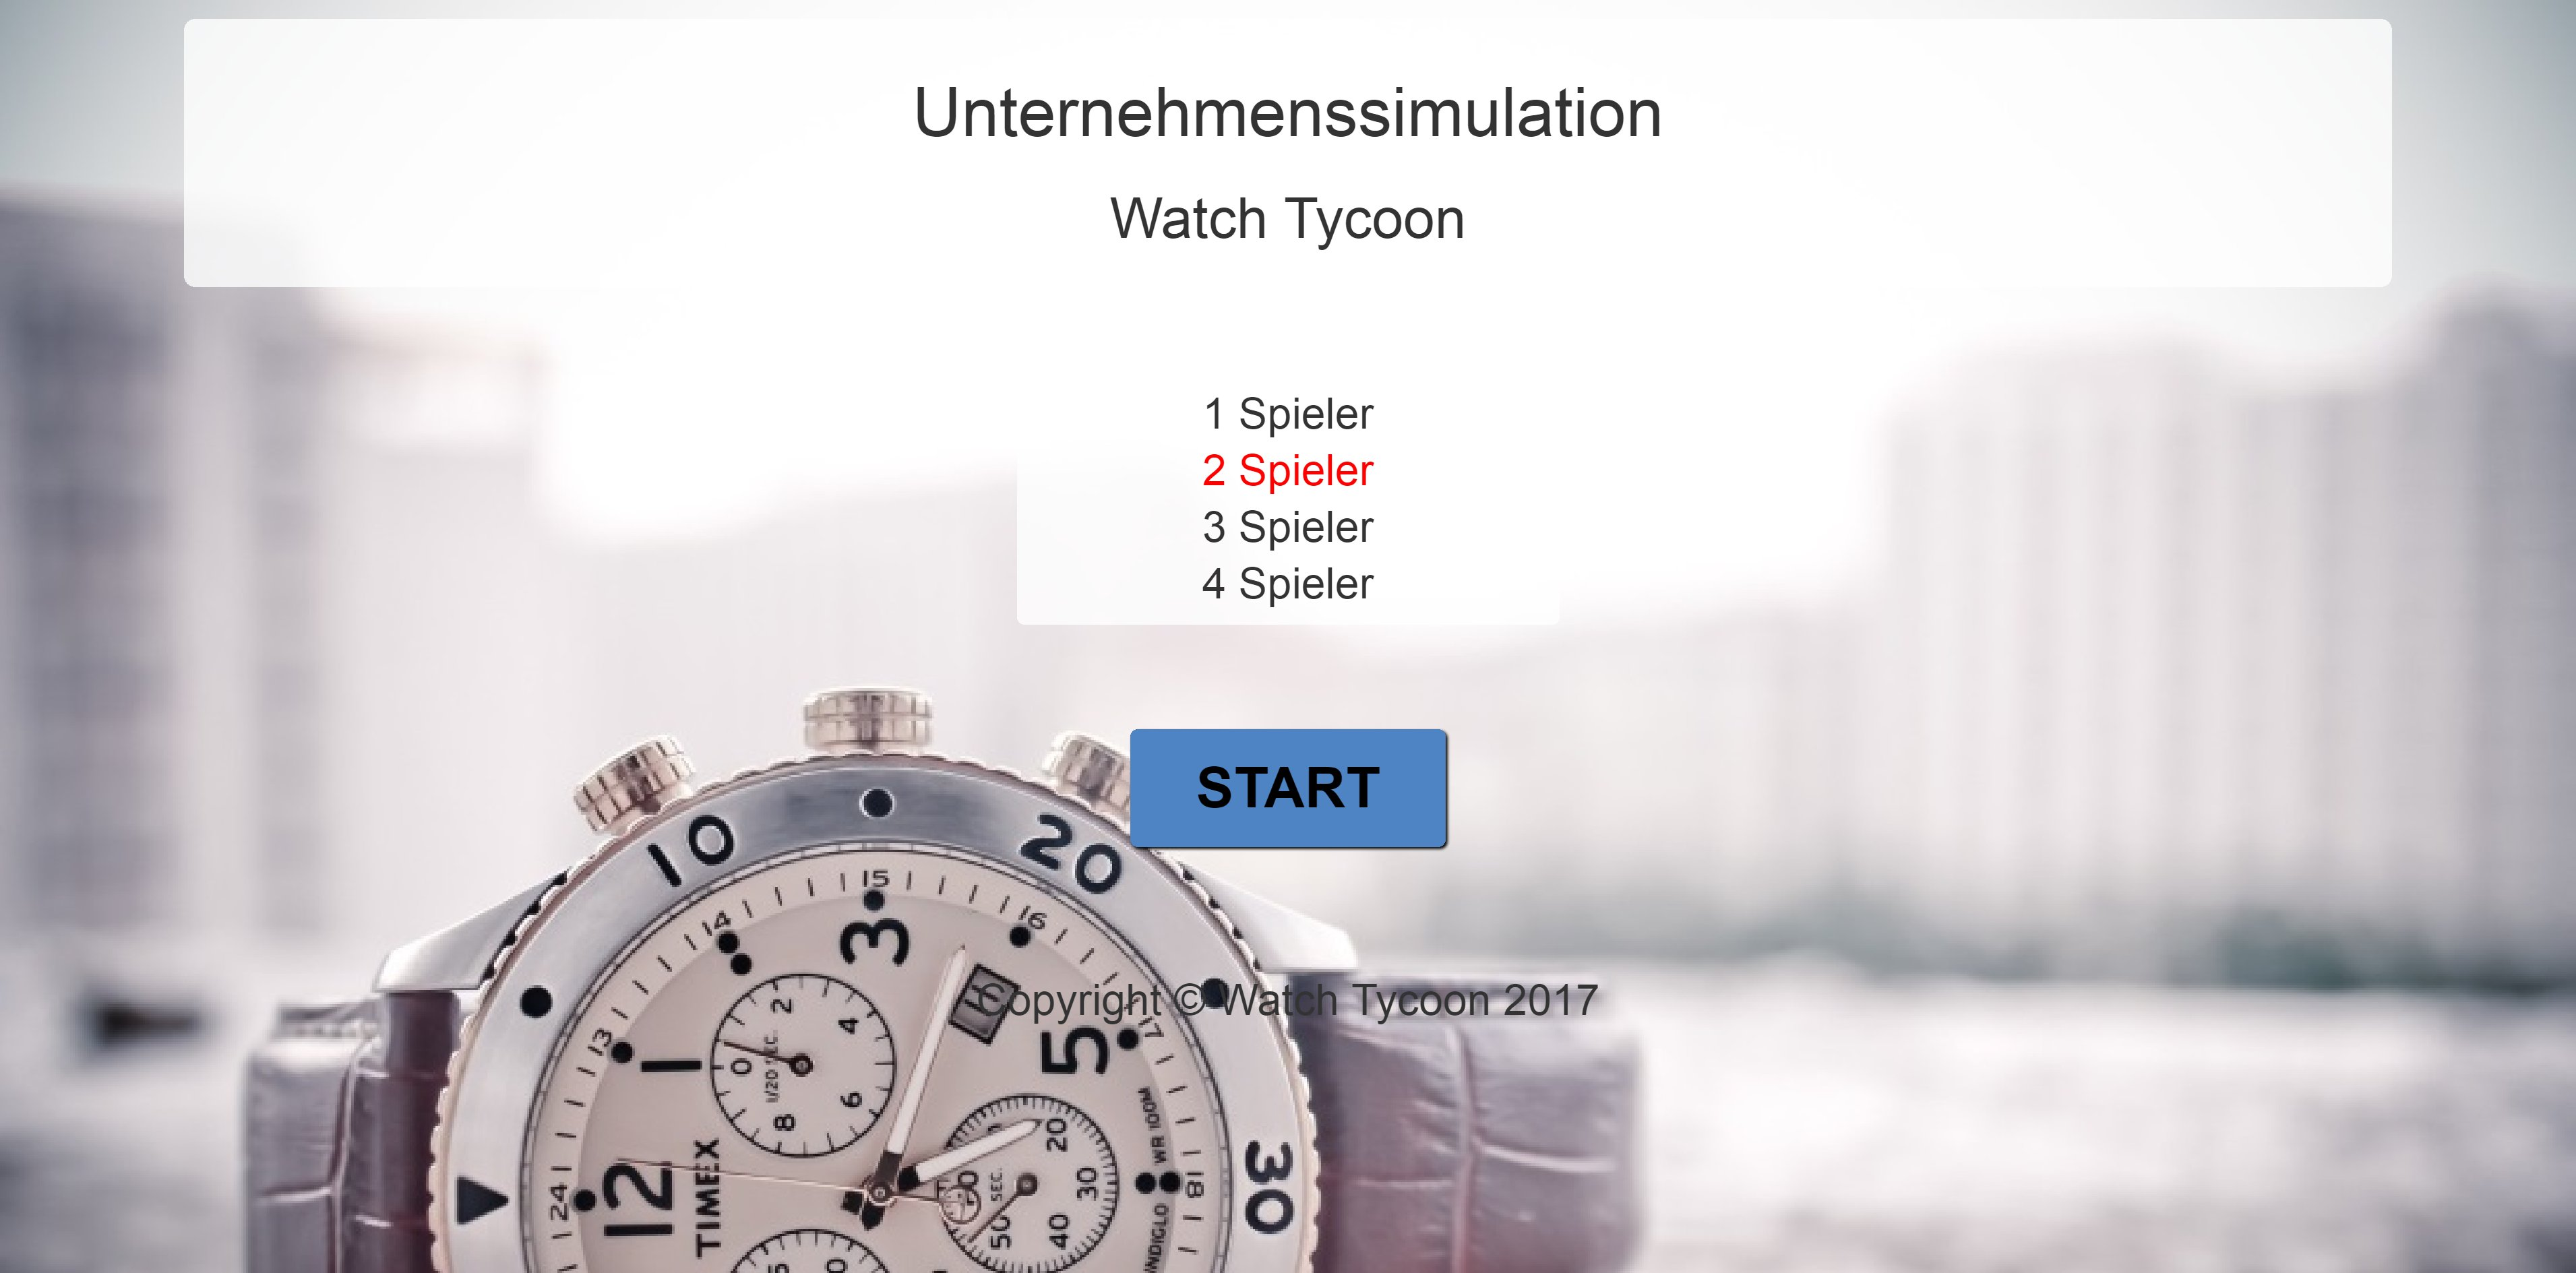
\includegraphics[scale=0.1]{img/bilder_layout/MockUp1.jpg}
	\label{fig:abb7}
	\caption{Mock-Up: Einstiegsbildschirm} 
\end{figure}
\begin{figure}
	\centering
	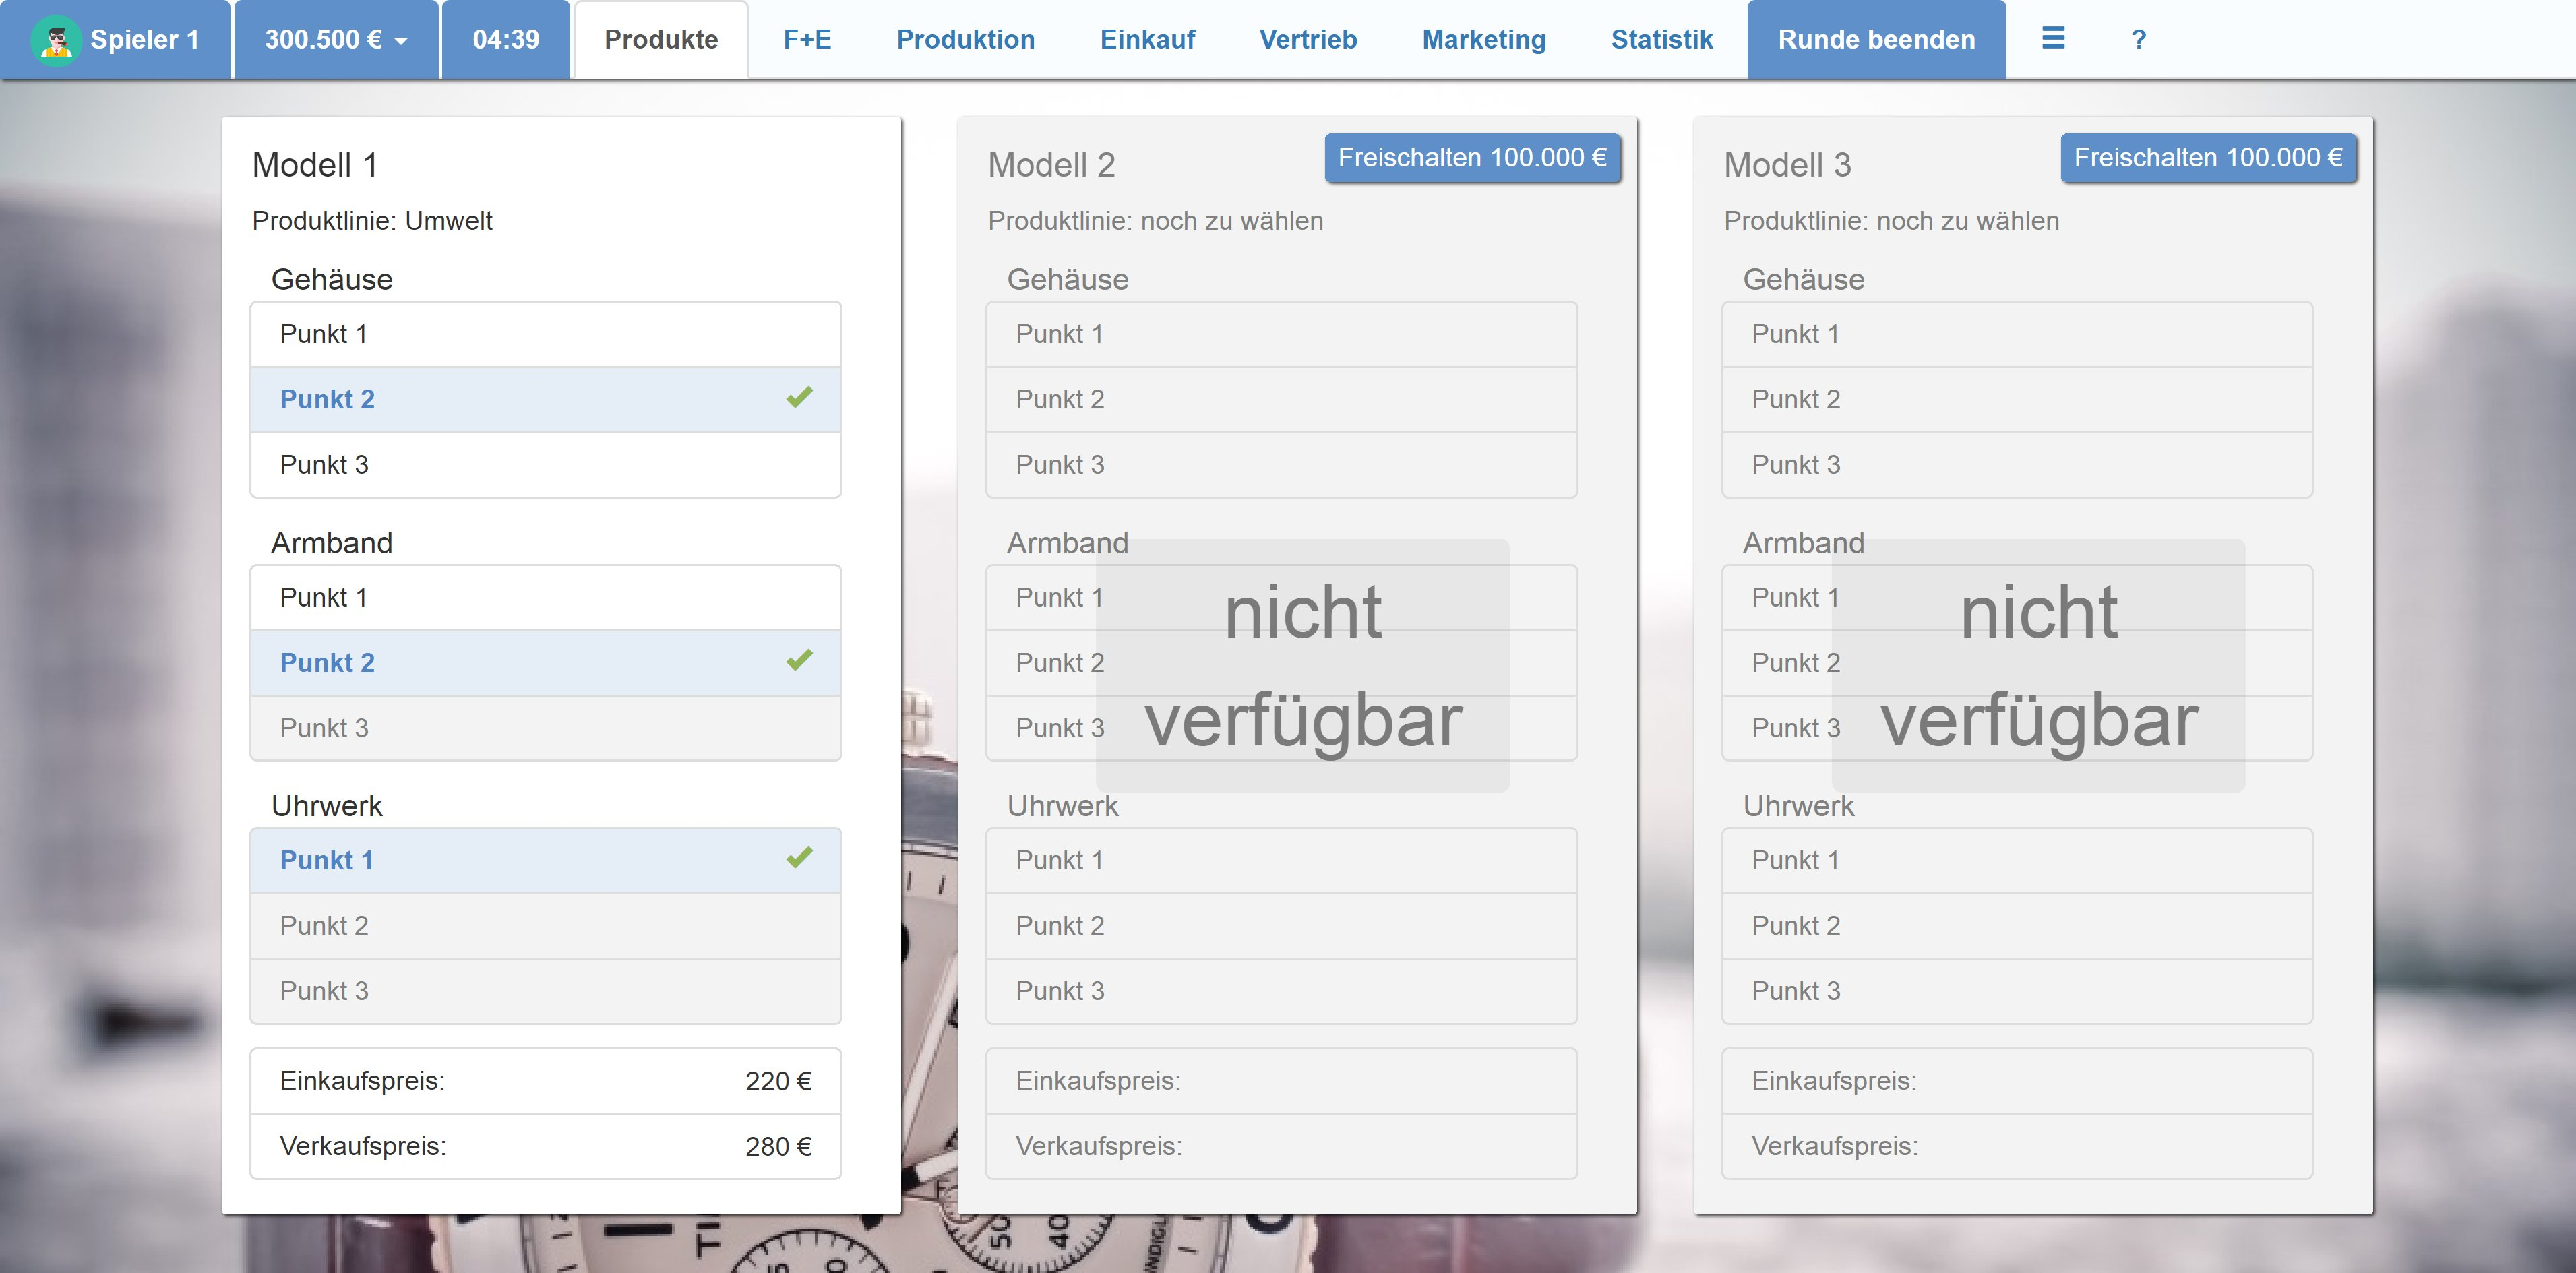
\includegraphics[scale=0.1]{img/bilder_layout/MockUp2.jpg}
	\label{fig:abb8}
	\caption{Mock-Up: Übersicht der Produkte} 
\end{figure}
\begin{figure} 
	\centering
	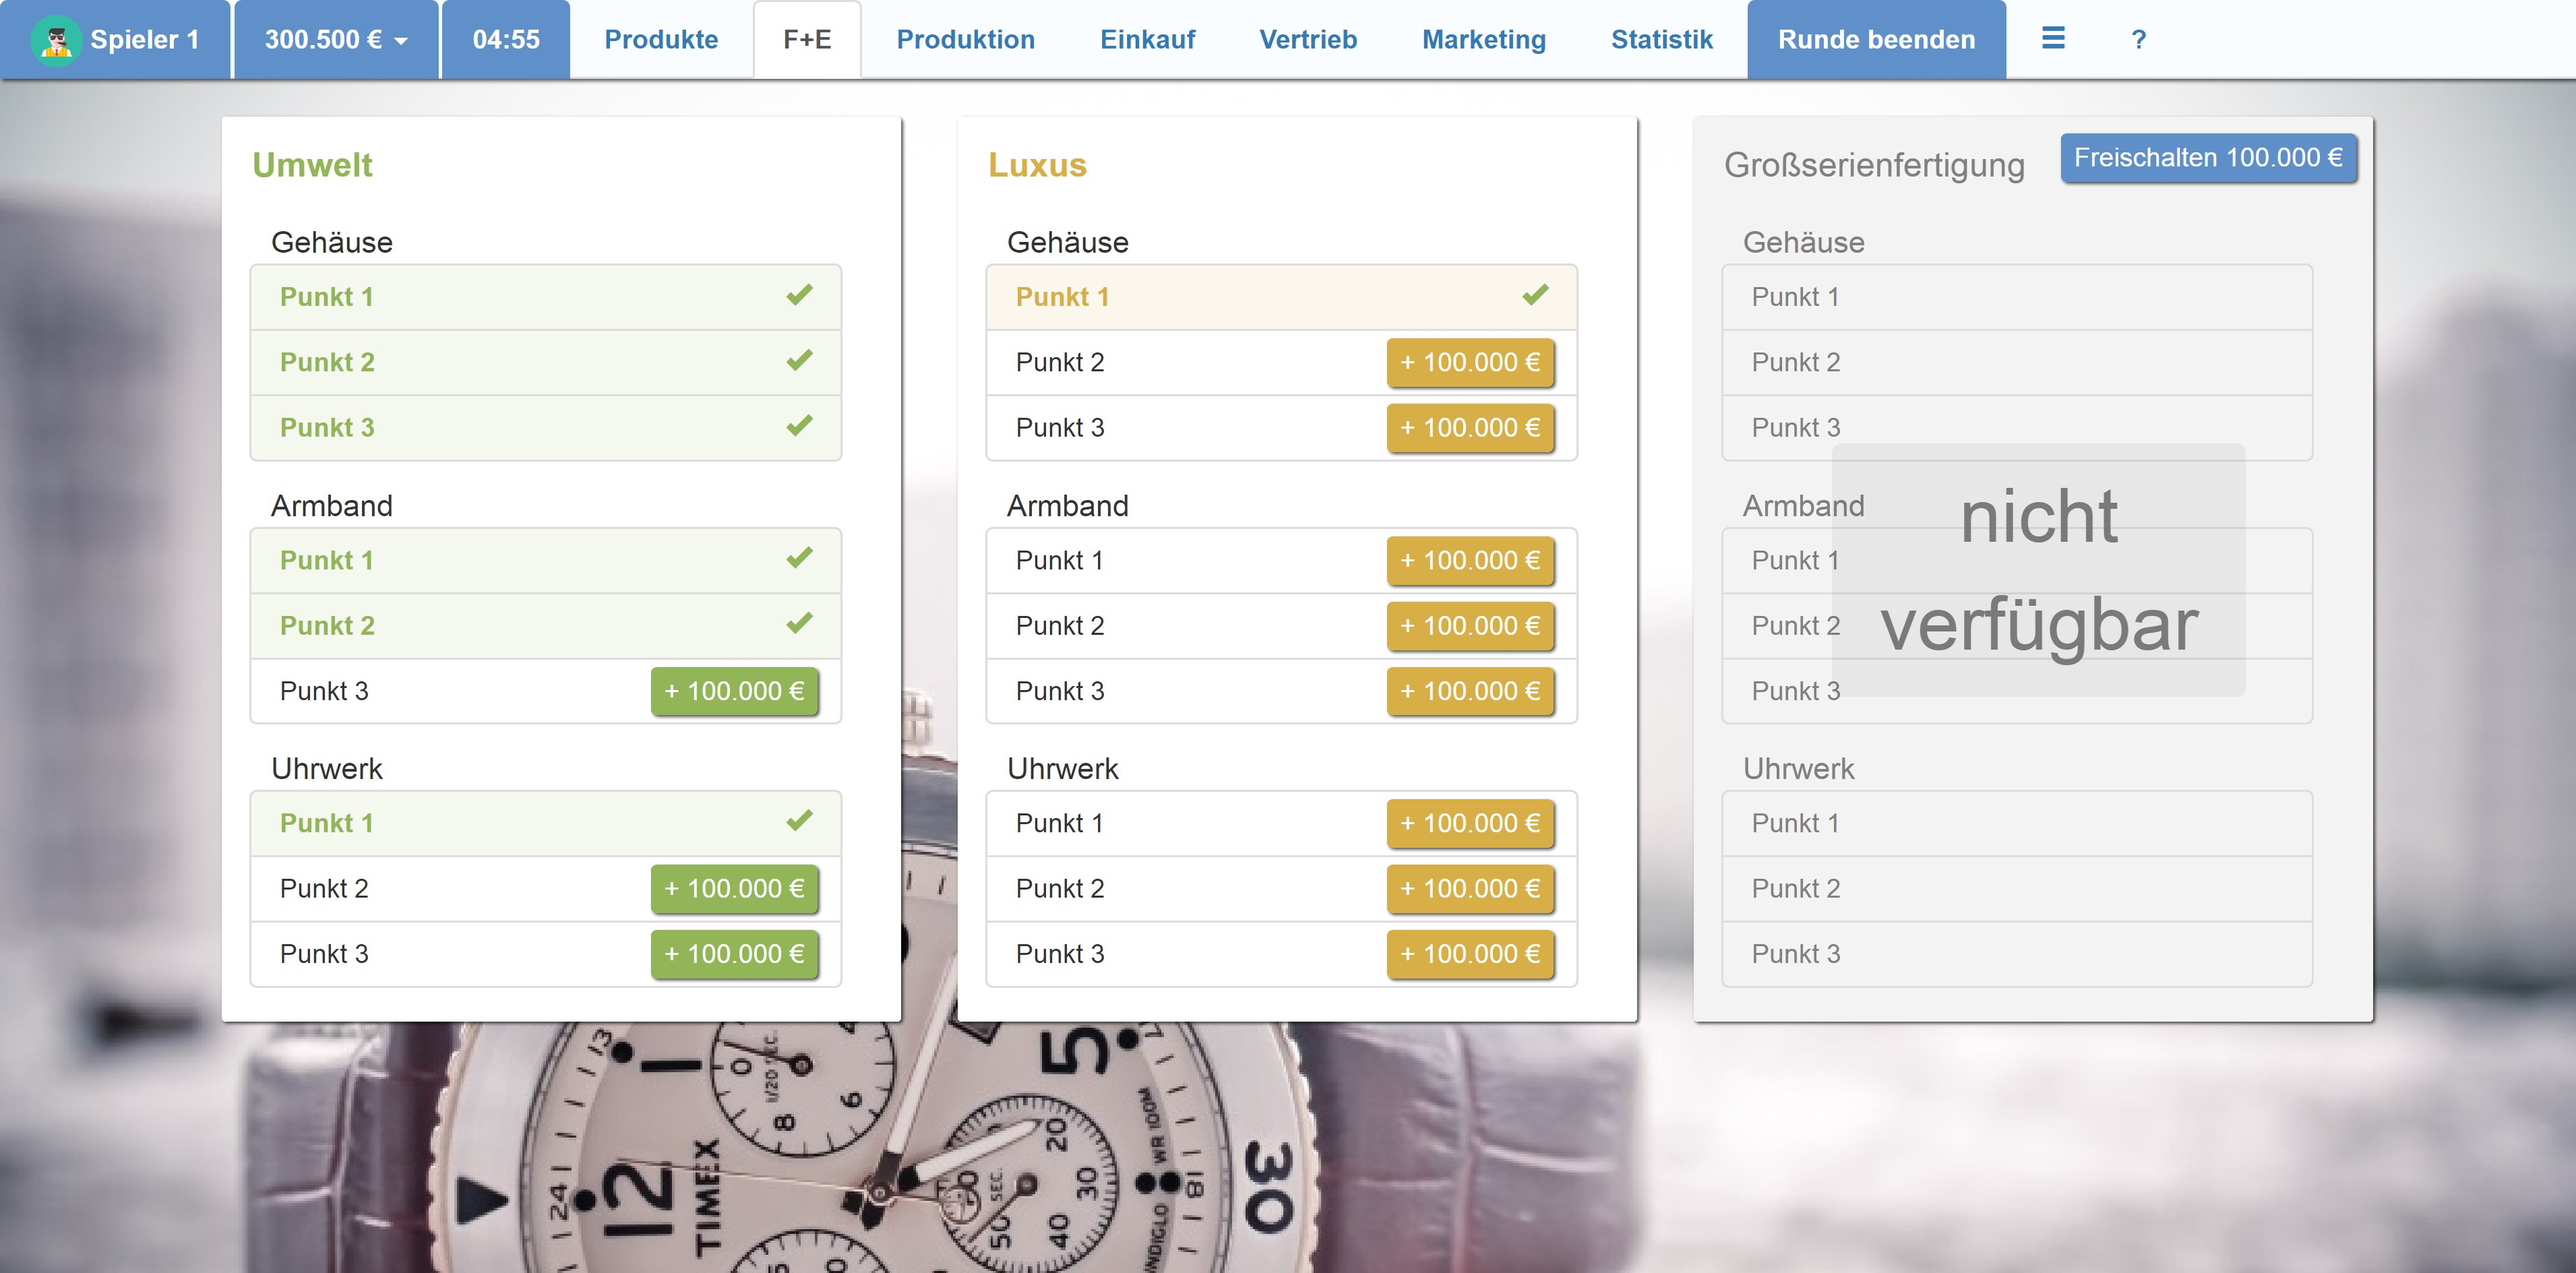
\includegraphics[scale=0.1]{img/bilder_layout/MockUp3.jpg}
	\label{fig:abb9}
	\caption{Mock-Up: Übersicht F\&E} 
\end{figure}
\begin{figure} 
	\centering
	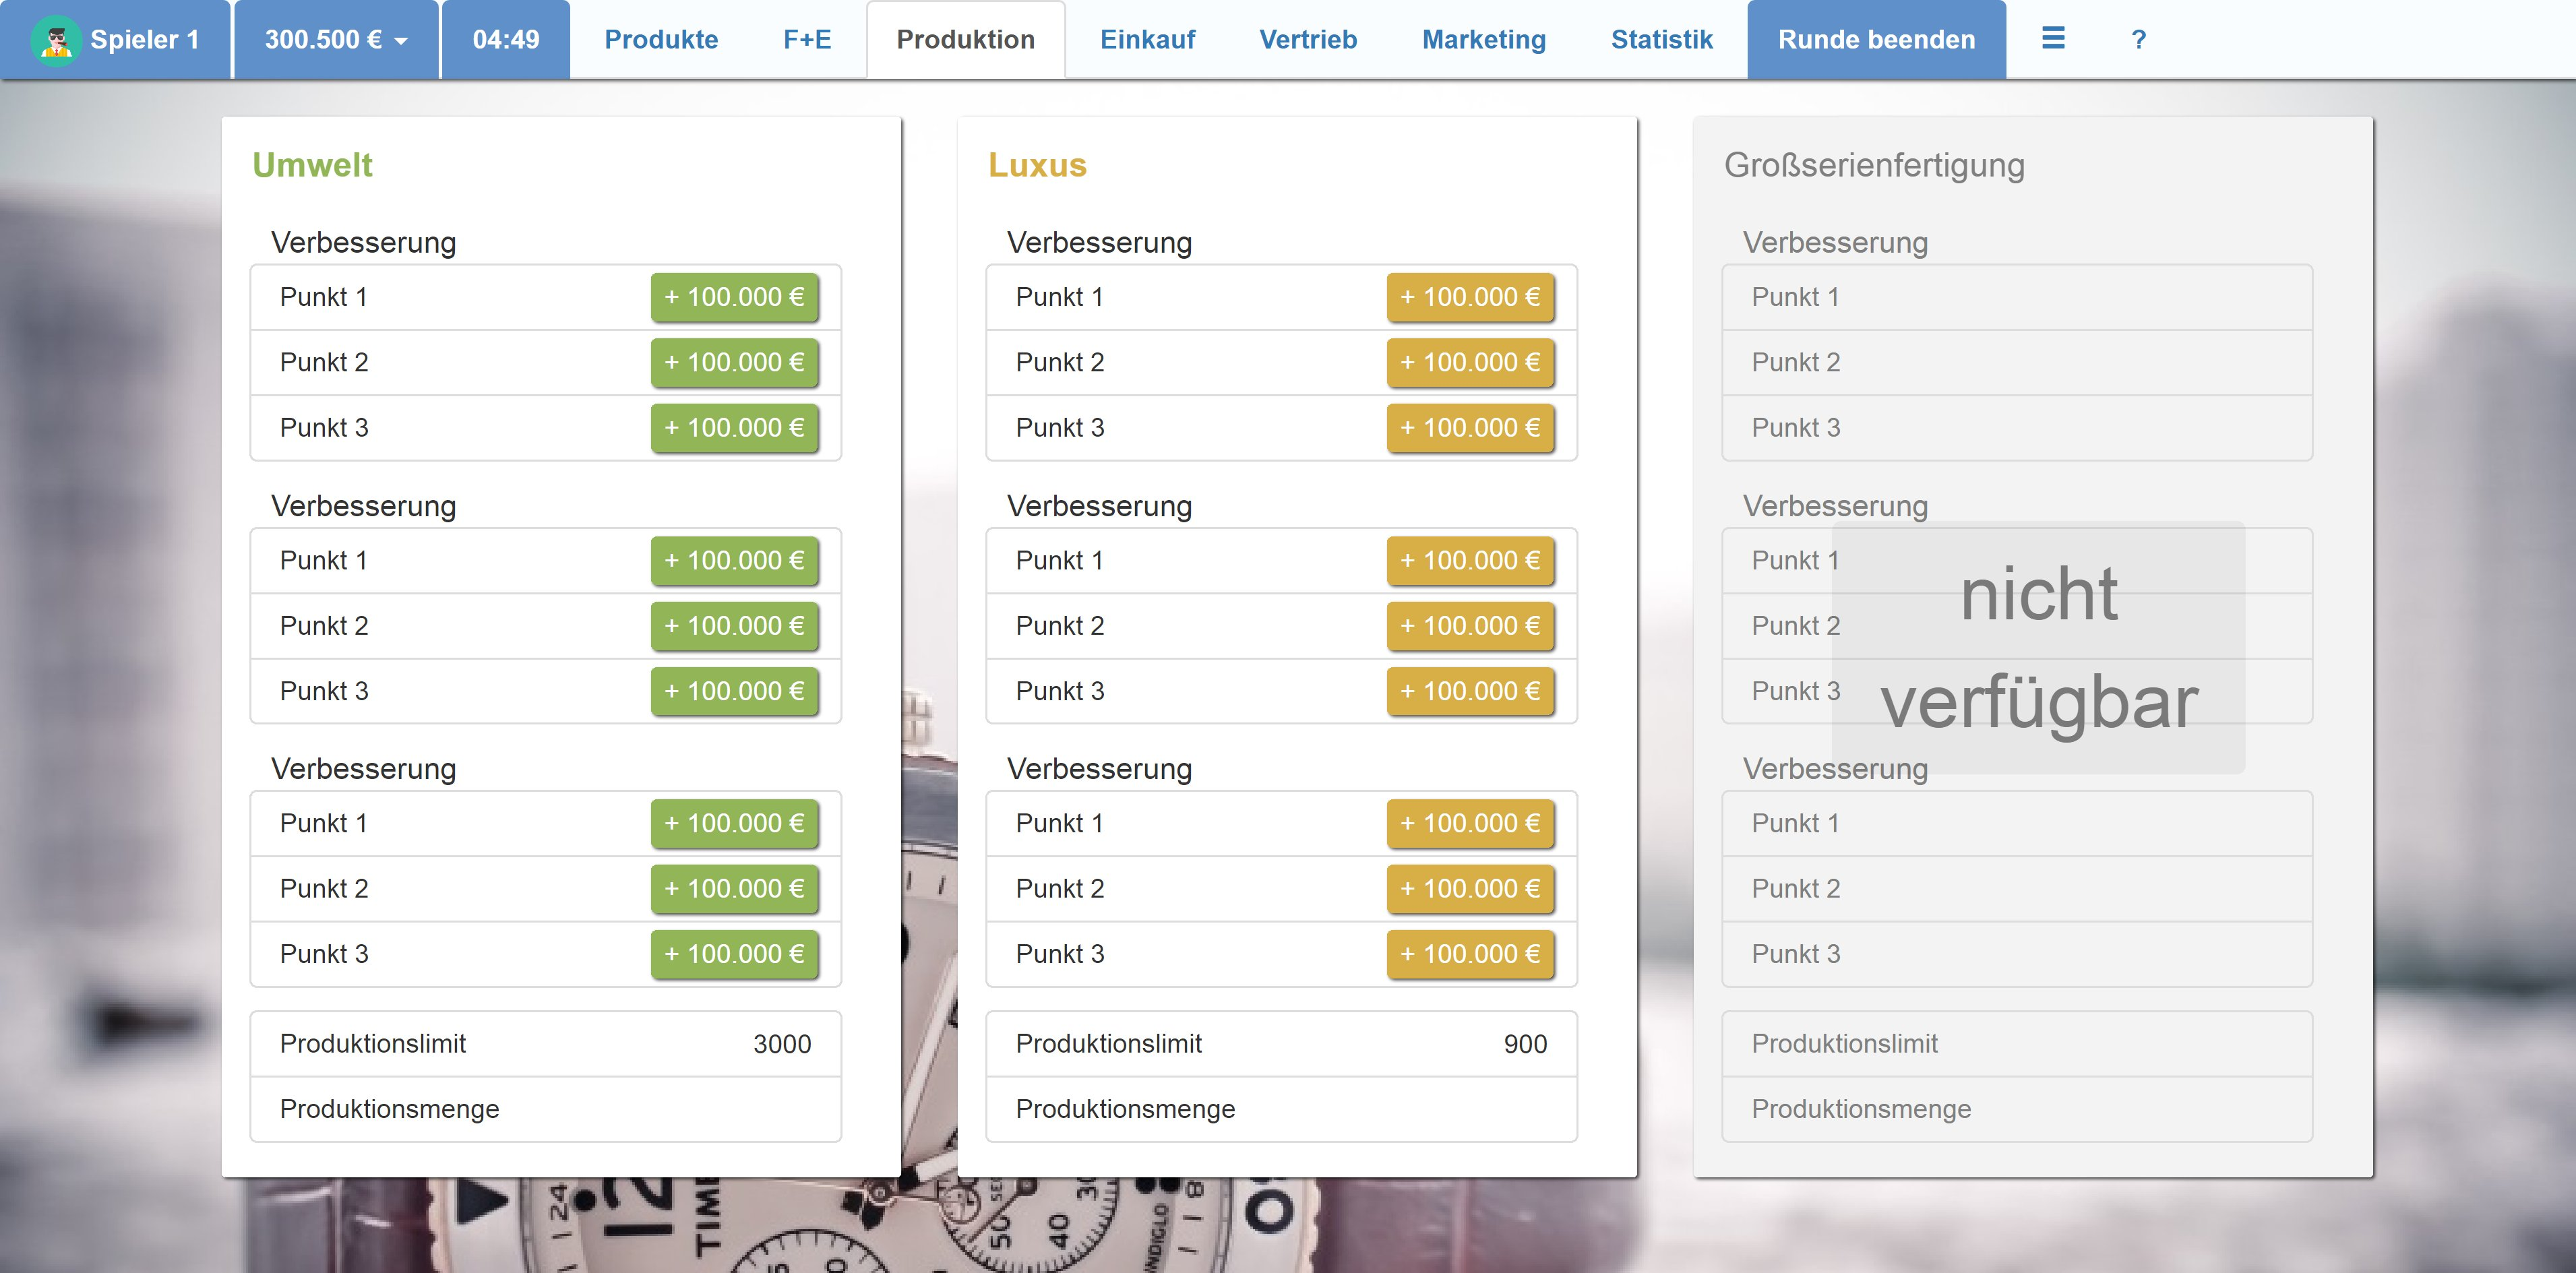
\includegraphics[scale=0.1]{img/bilder_layout/MockUp4.jpg}
	\label{fig:abb10}
	\caption{Mock-Up: Übersicht Produktion} 
\end{figure}
\begin{figure} 
	\centering
	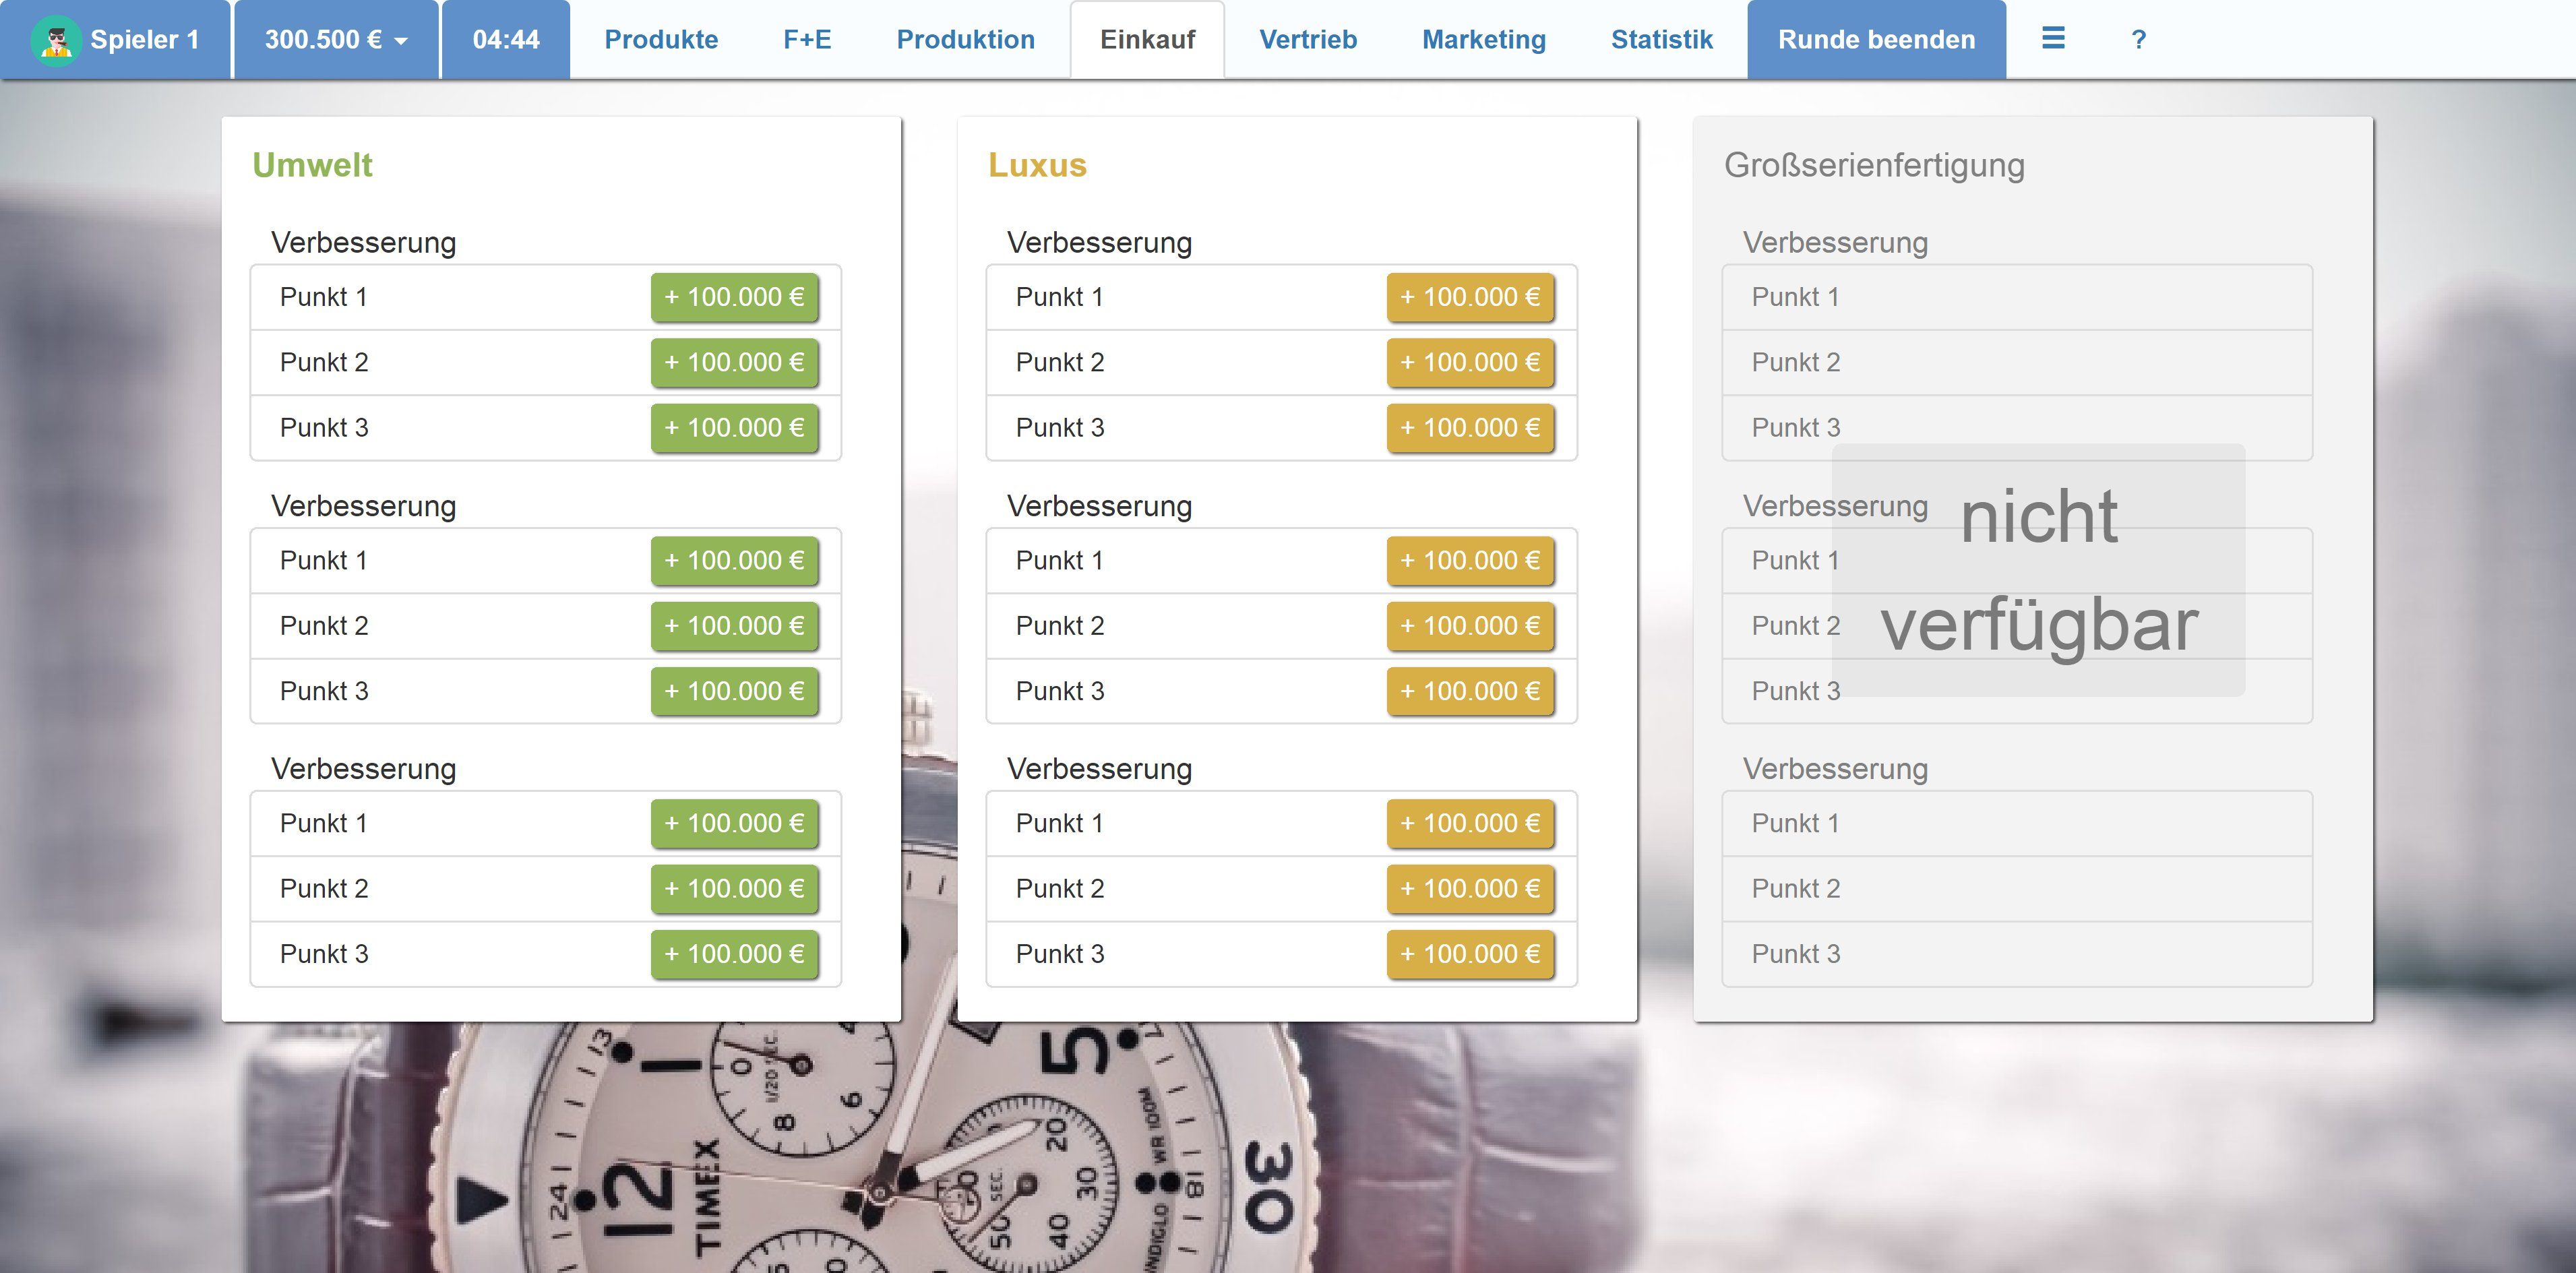
\includegraphics[scale=0.1]{img/bilder_layout/MockUp6.jpg}
	\label{fig:abb11}
	\caption{Mock-Up: Übersicht Einkauf} 
\end{figure}
\begin{figure} 
	\centering
	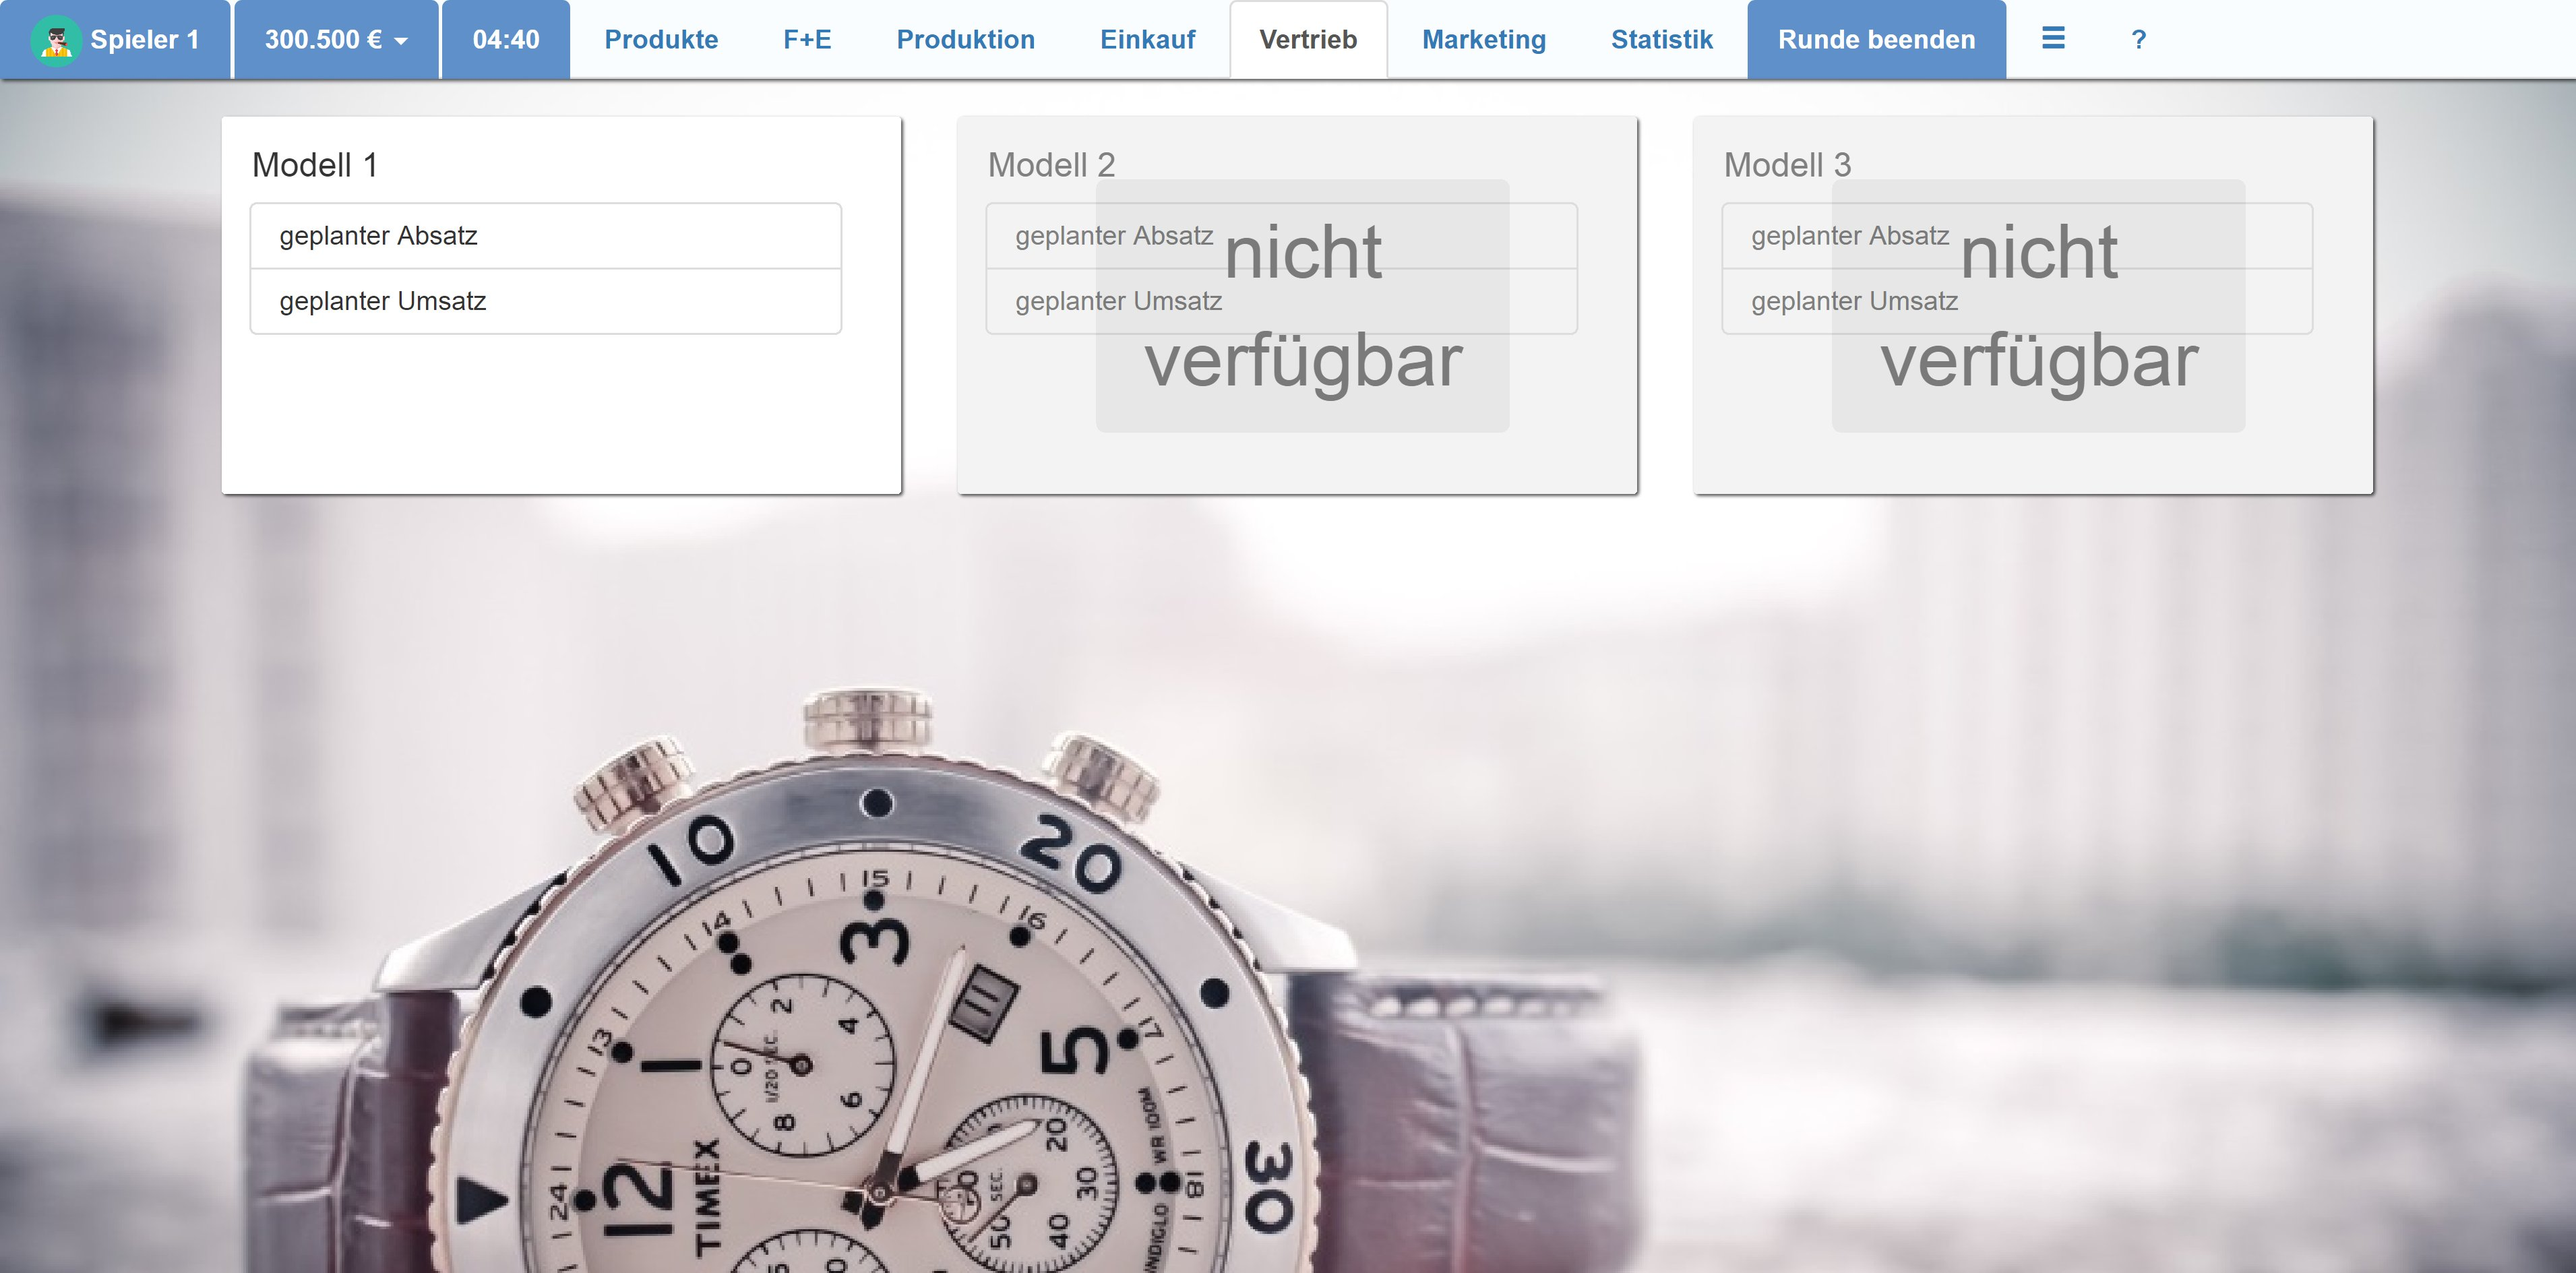
\includegraphics[scale=0.1]{img/bilder_layout/MockUp7.jpg}
	\label{fig:abb12}
	\caption{Mock-Up: Übersicht Vertrieb} 
\end{figure}
\begin{figure} 
	\centering
	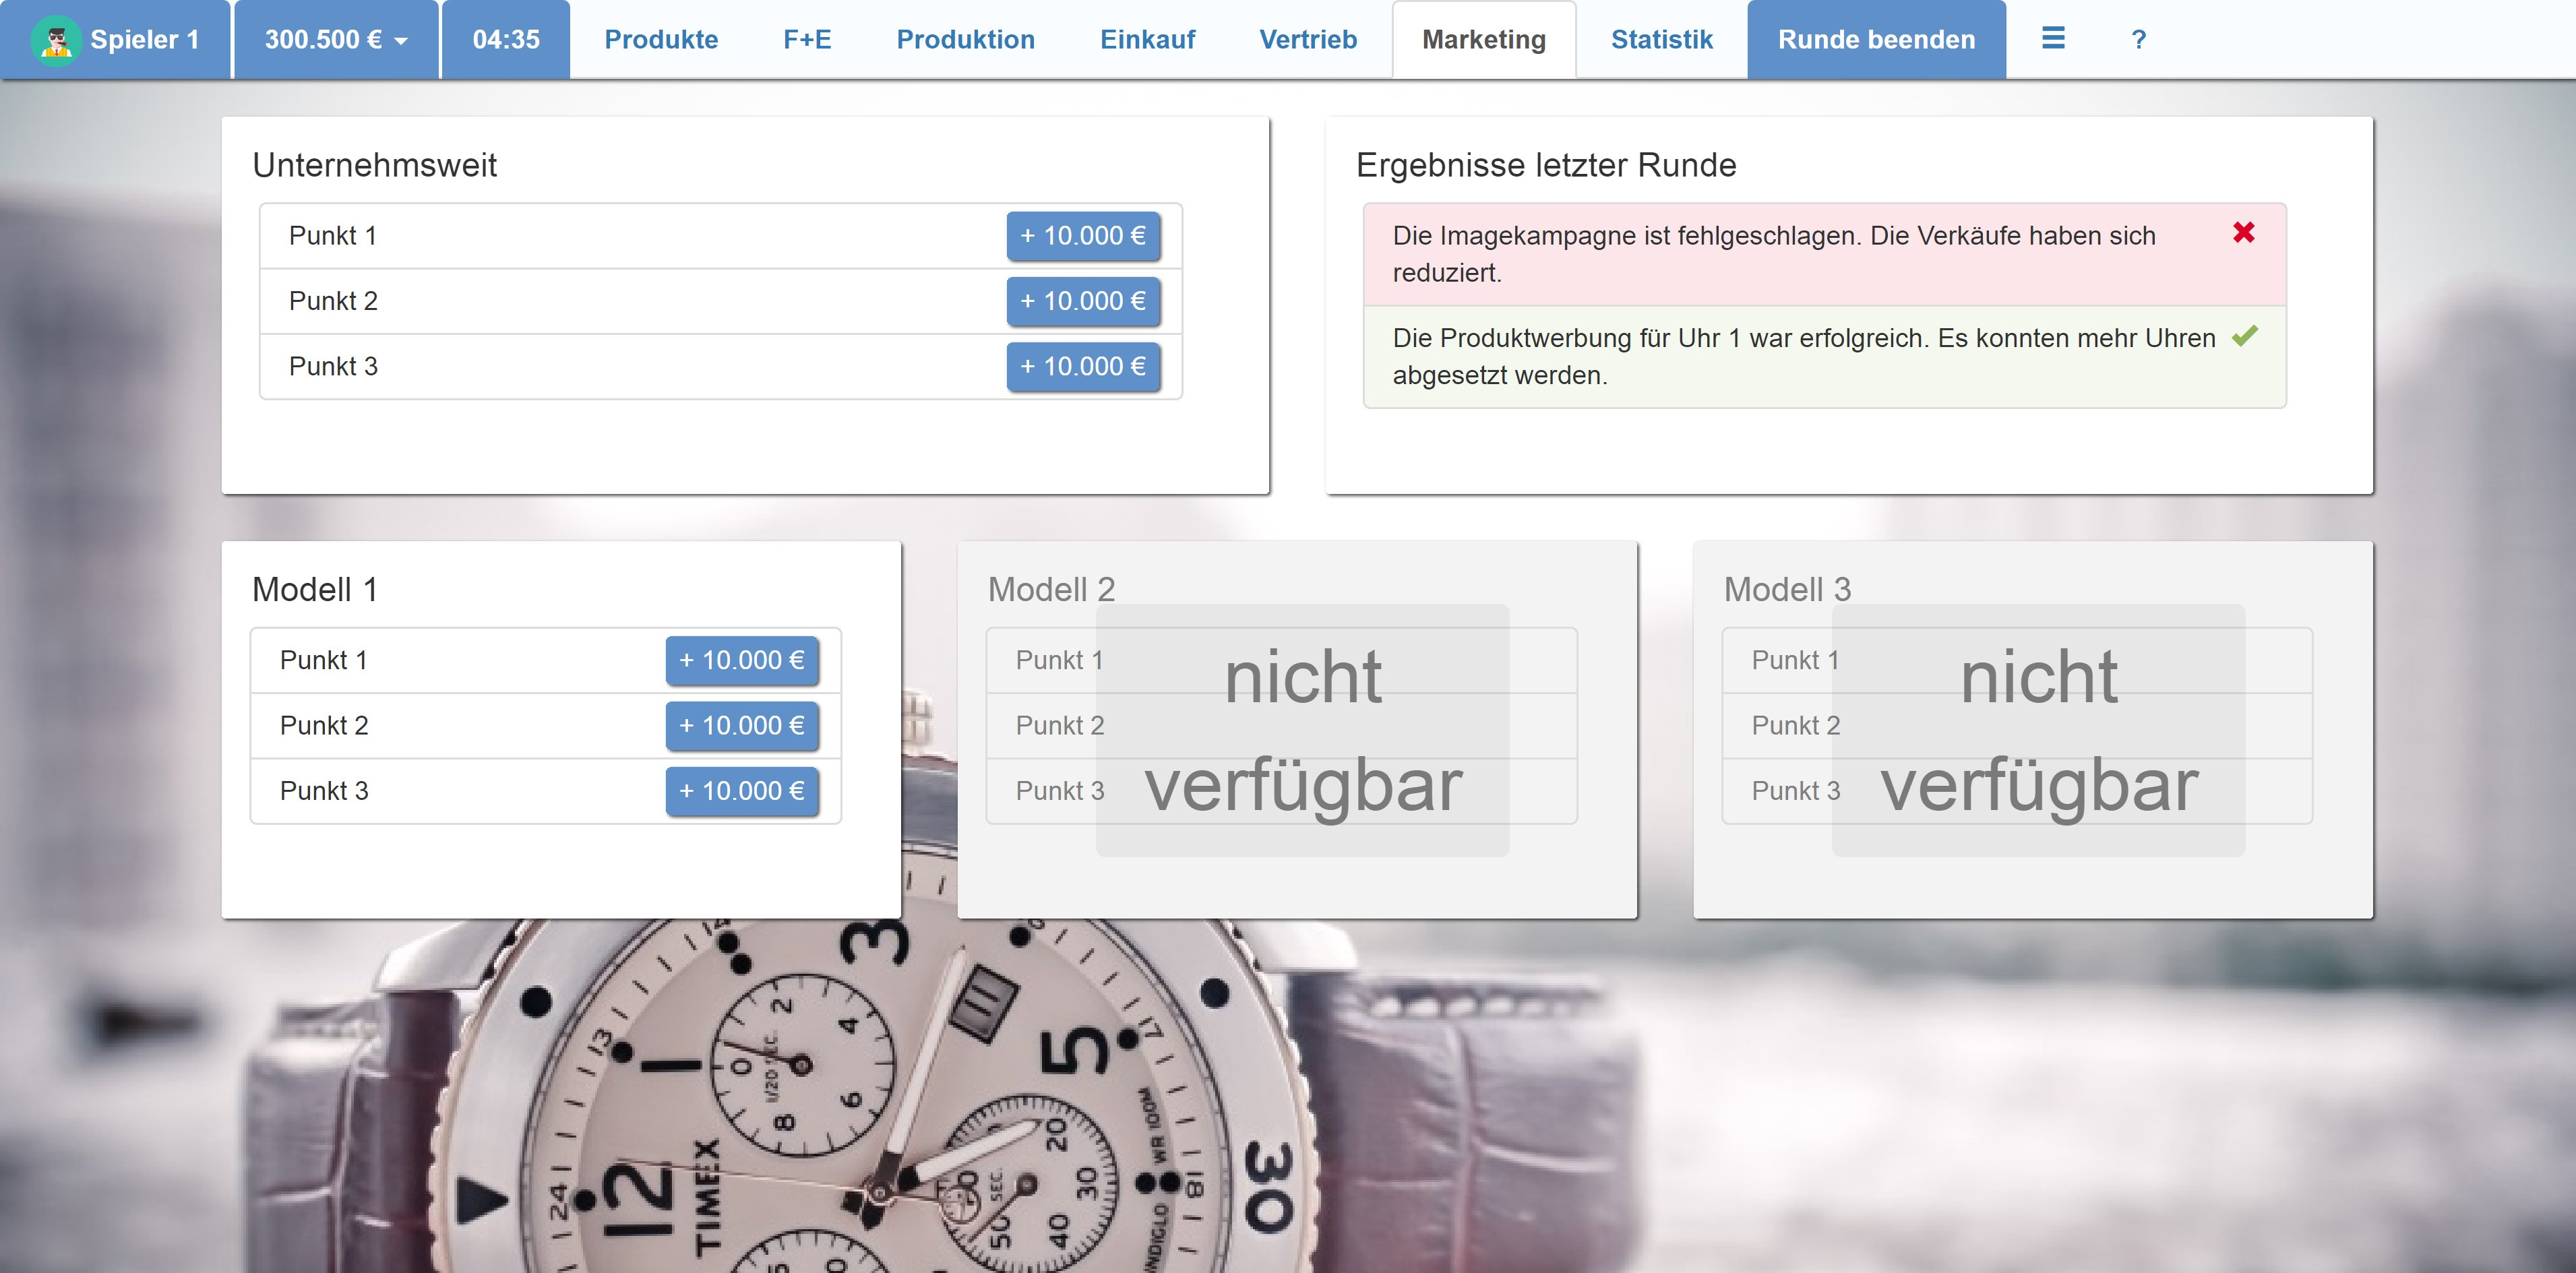
\includegraphics[scale=0.1]{img/bilder_layout/MockUp9.jpg}
	\label{fig:abb13}
	\caption{Mock-Up: Übersicht Marketing} 
\end{figure}
\begin{figure} 
	\centering
	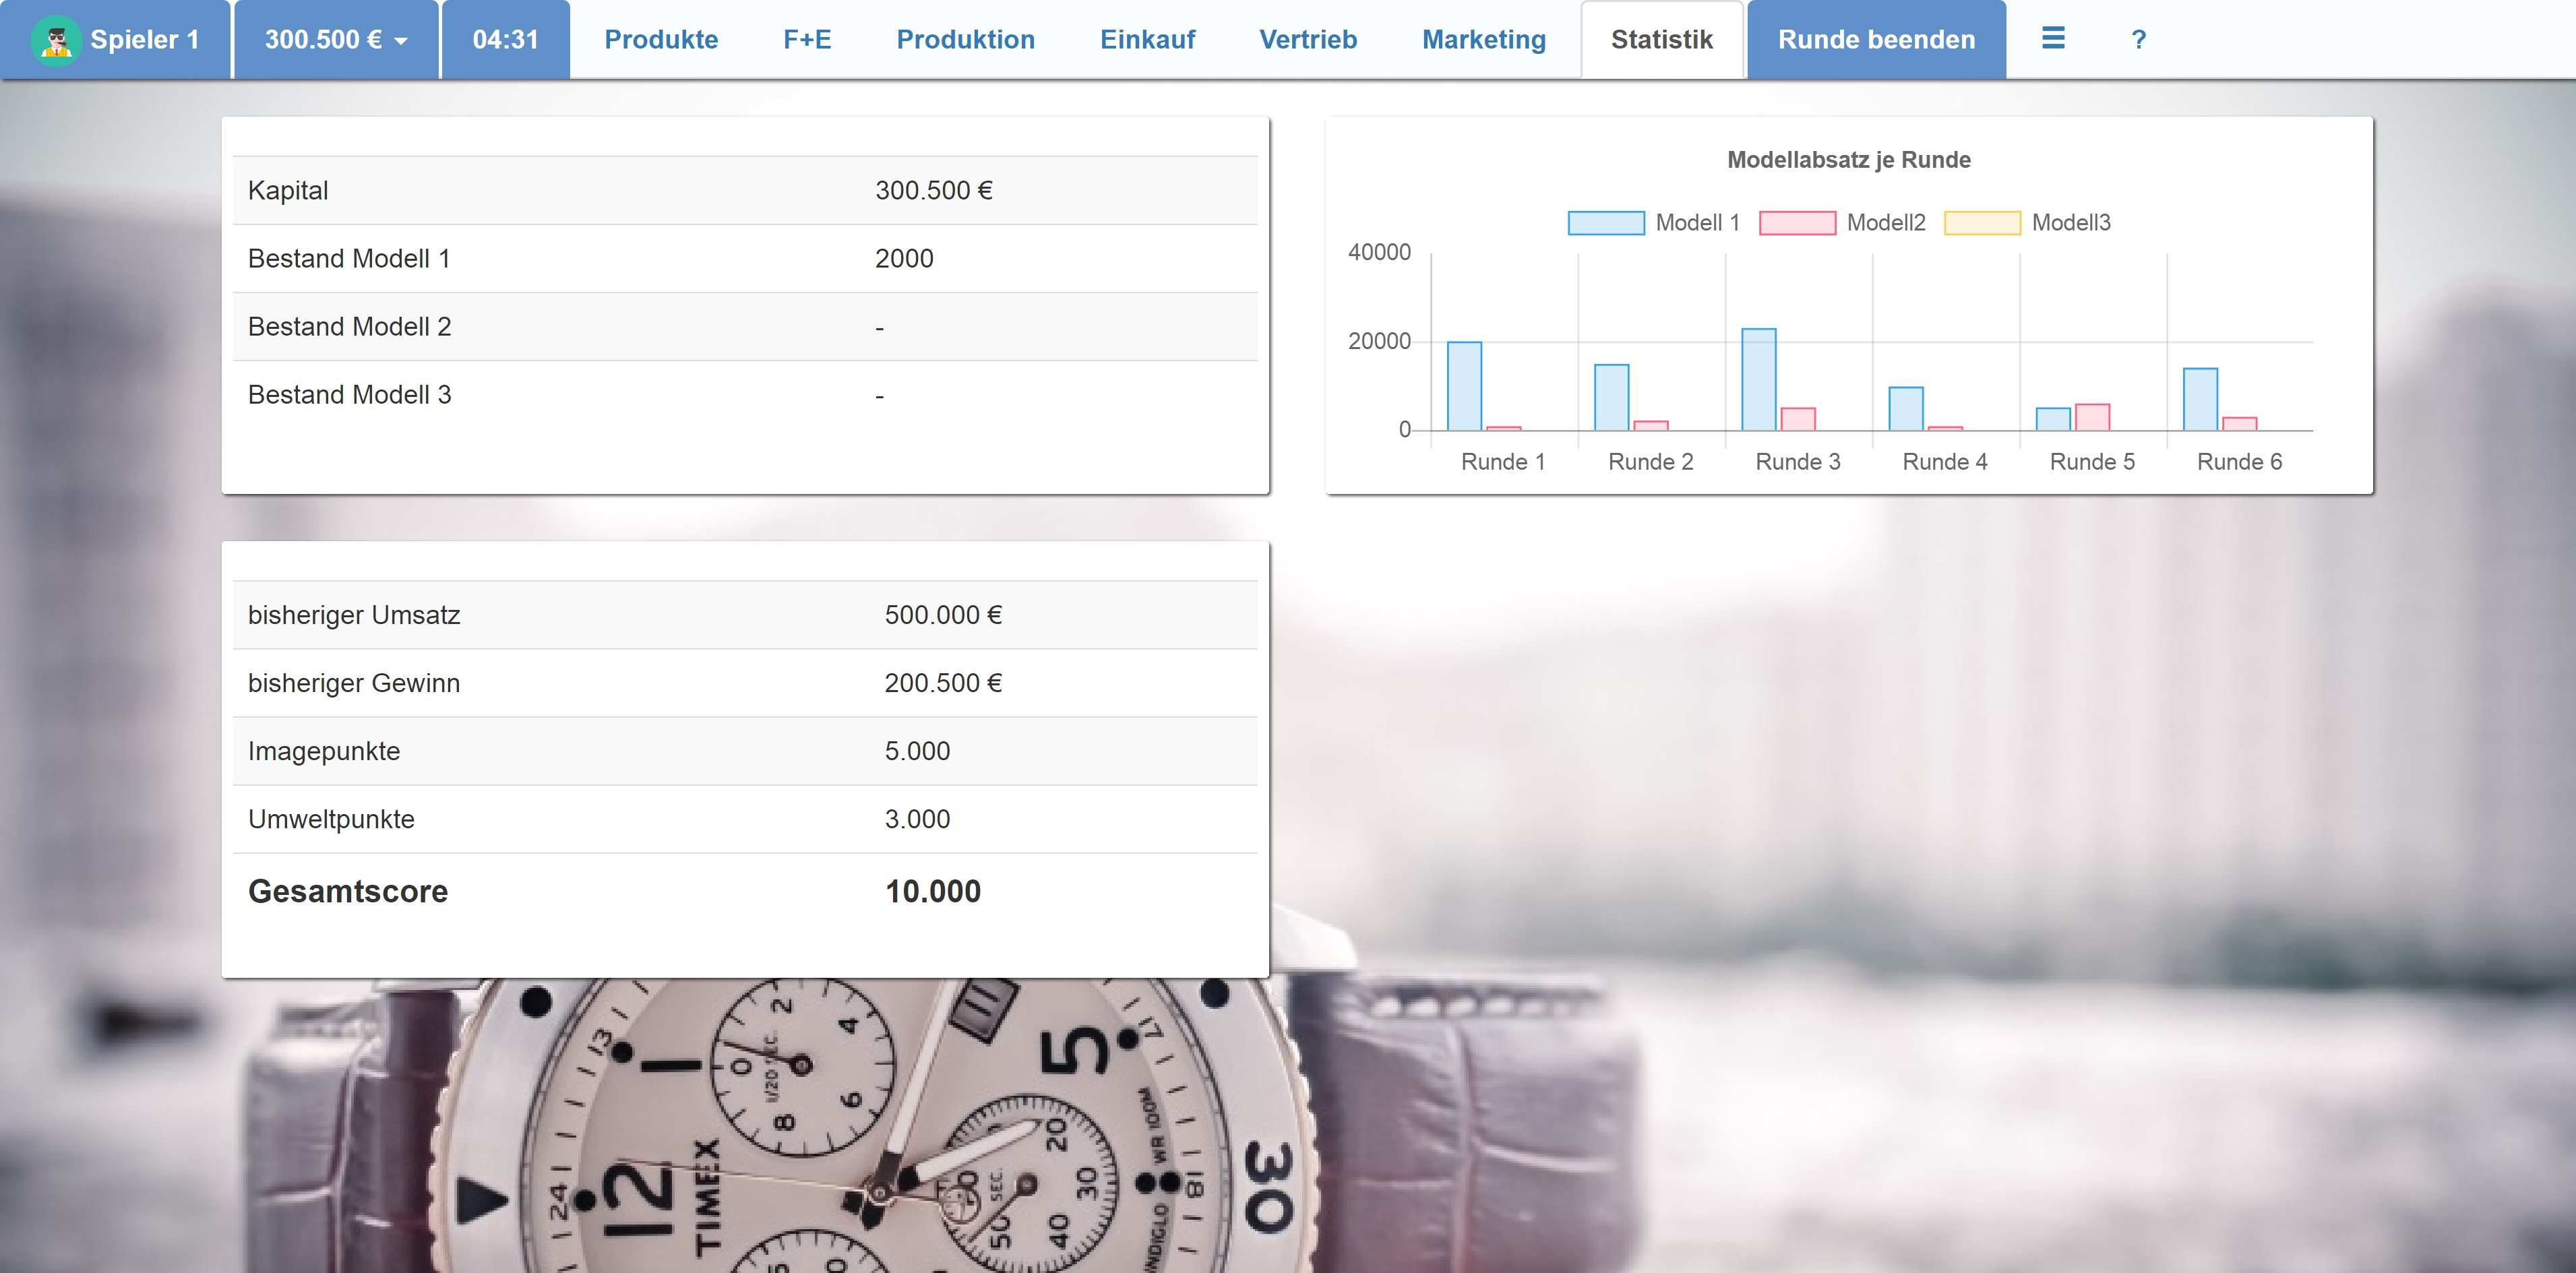
\includegraphics[scale=0.1]{img/bilder_layout/MockUp5.jpg}
	\label{fig:abb14}
	\caption{Mock-Up: Übersicht Statistik/Markt} 
\end{figure}
\begin{figure} 
	\centering
	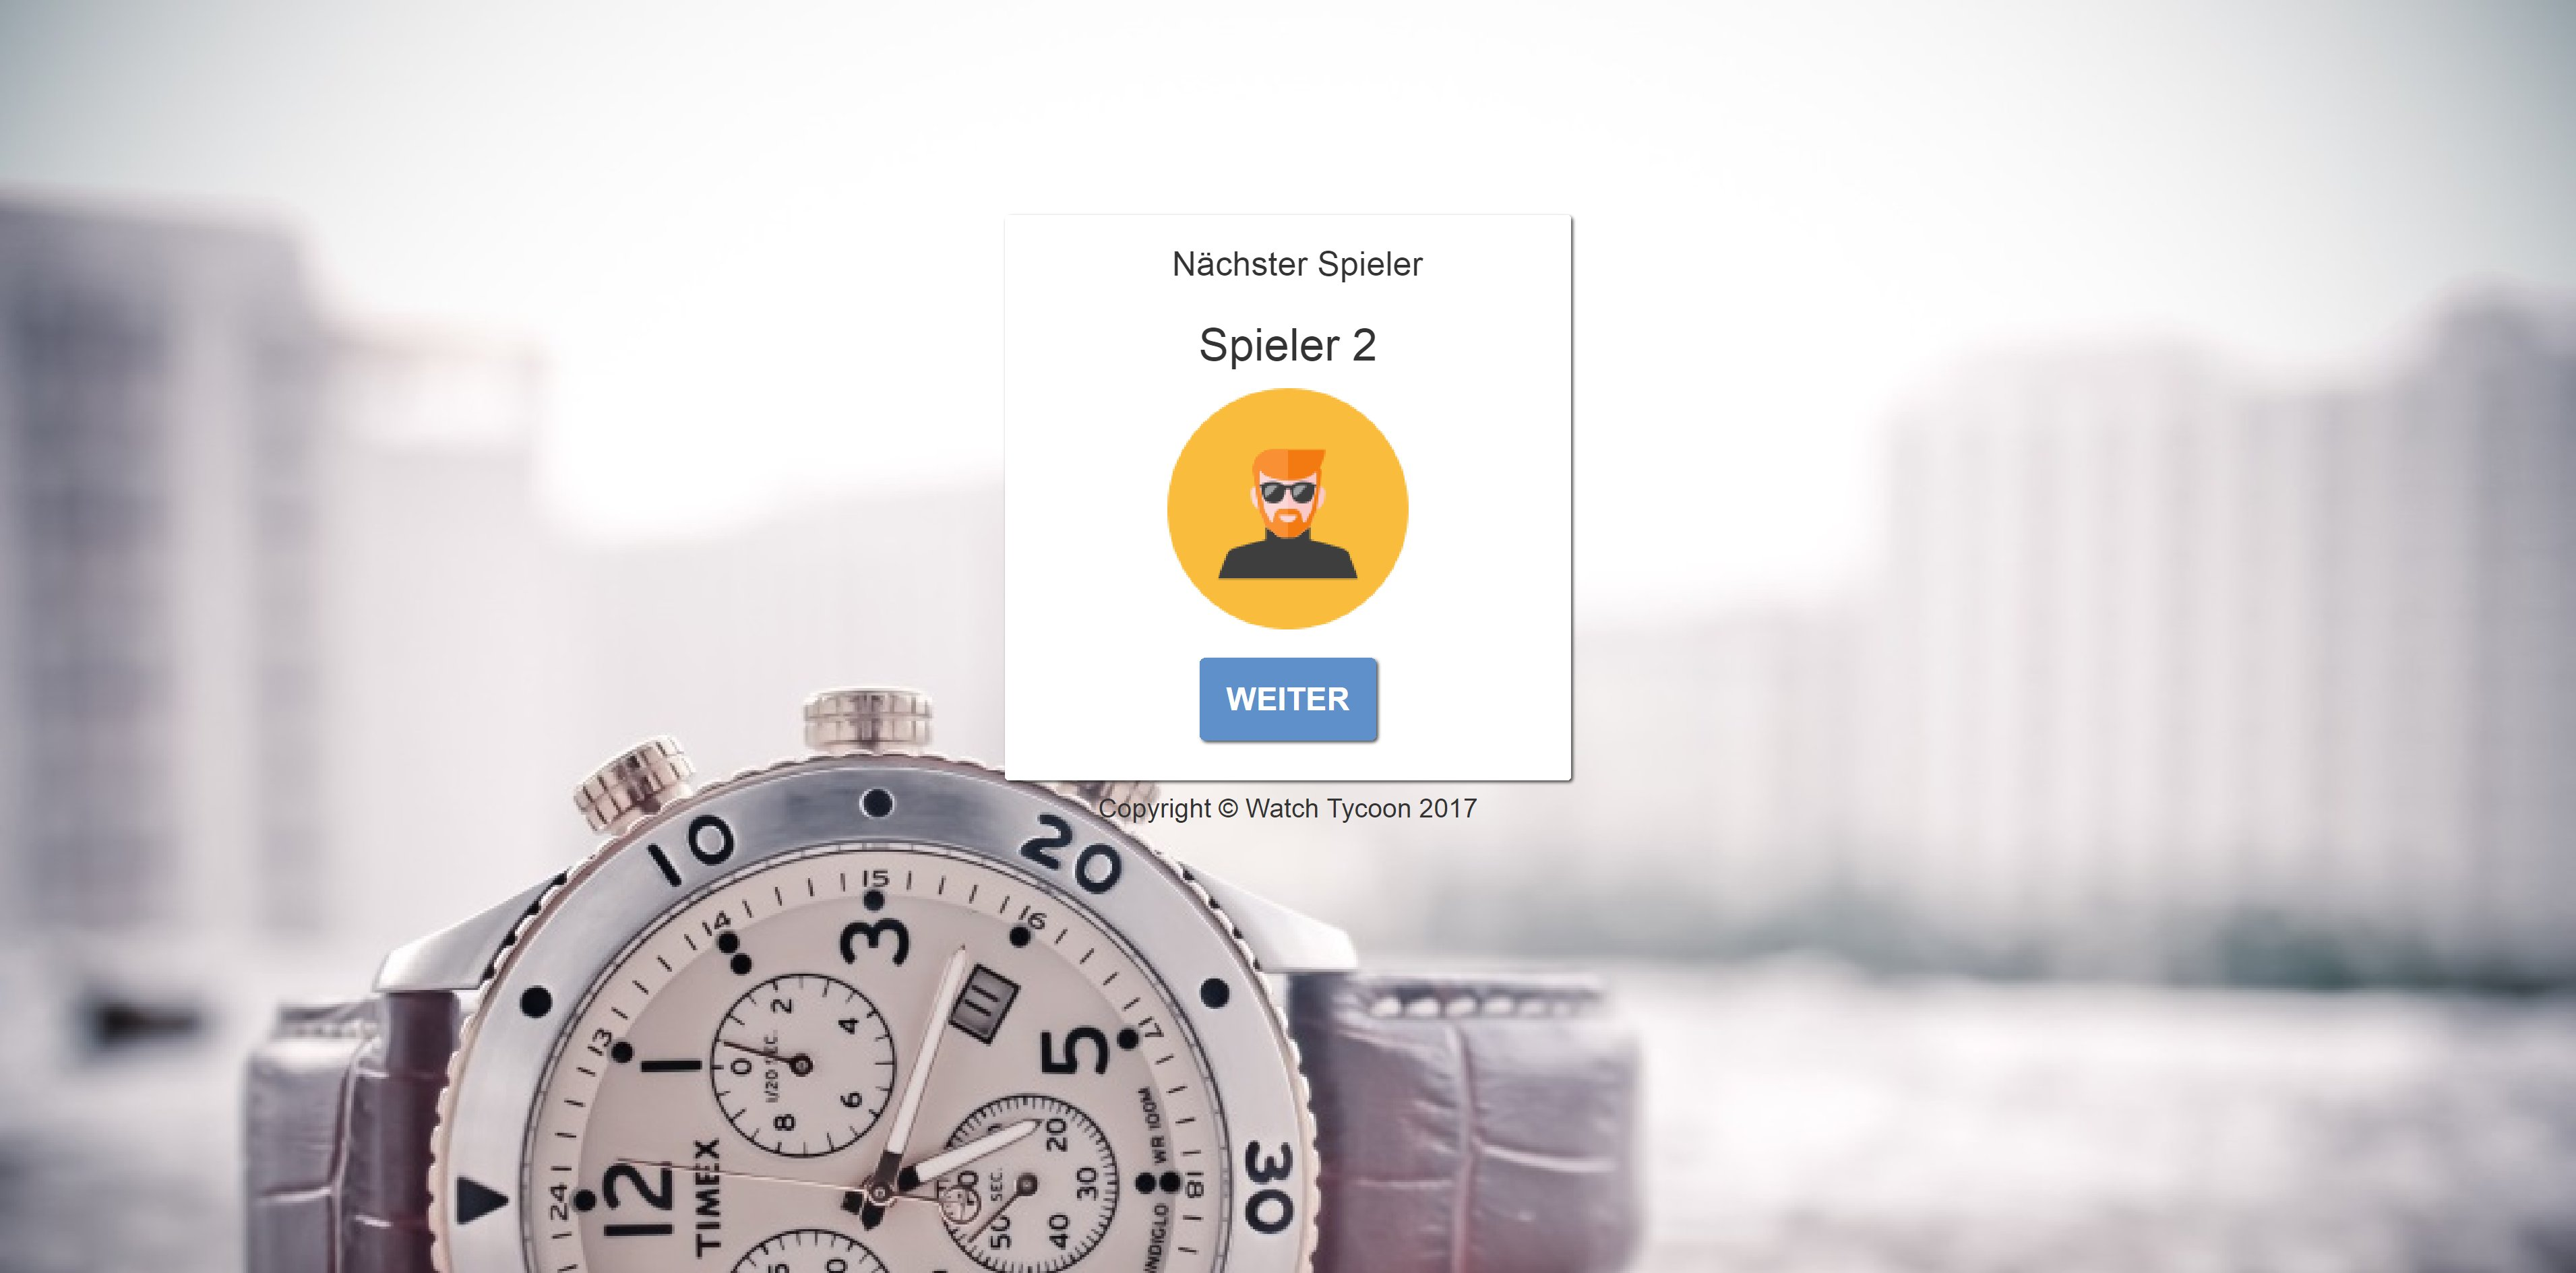
\includegraphics[scale=0.1]{img/bilder_layout/MockUp8.jpg} \label{fig:abb15}
	\caption{Mock-Up: \enquote{Nächster Spieler}-Anzeige} 
\end{figure}



\clearpage
\section{Finales UI}\label{sec:final_UI} 
\begin{figure} [!h]
\begin{minipage}{\textwidth} 
Der Einstiegsbildschirm zeigt die Auswahl der Spieleranzahl und startet mit einem Klick auf \enquote{START} direkt mit dem Spiel und Spieler1.\\
\end{minipage}
	\centering
	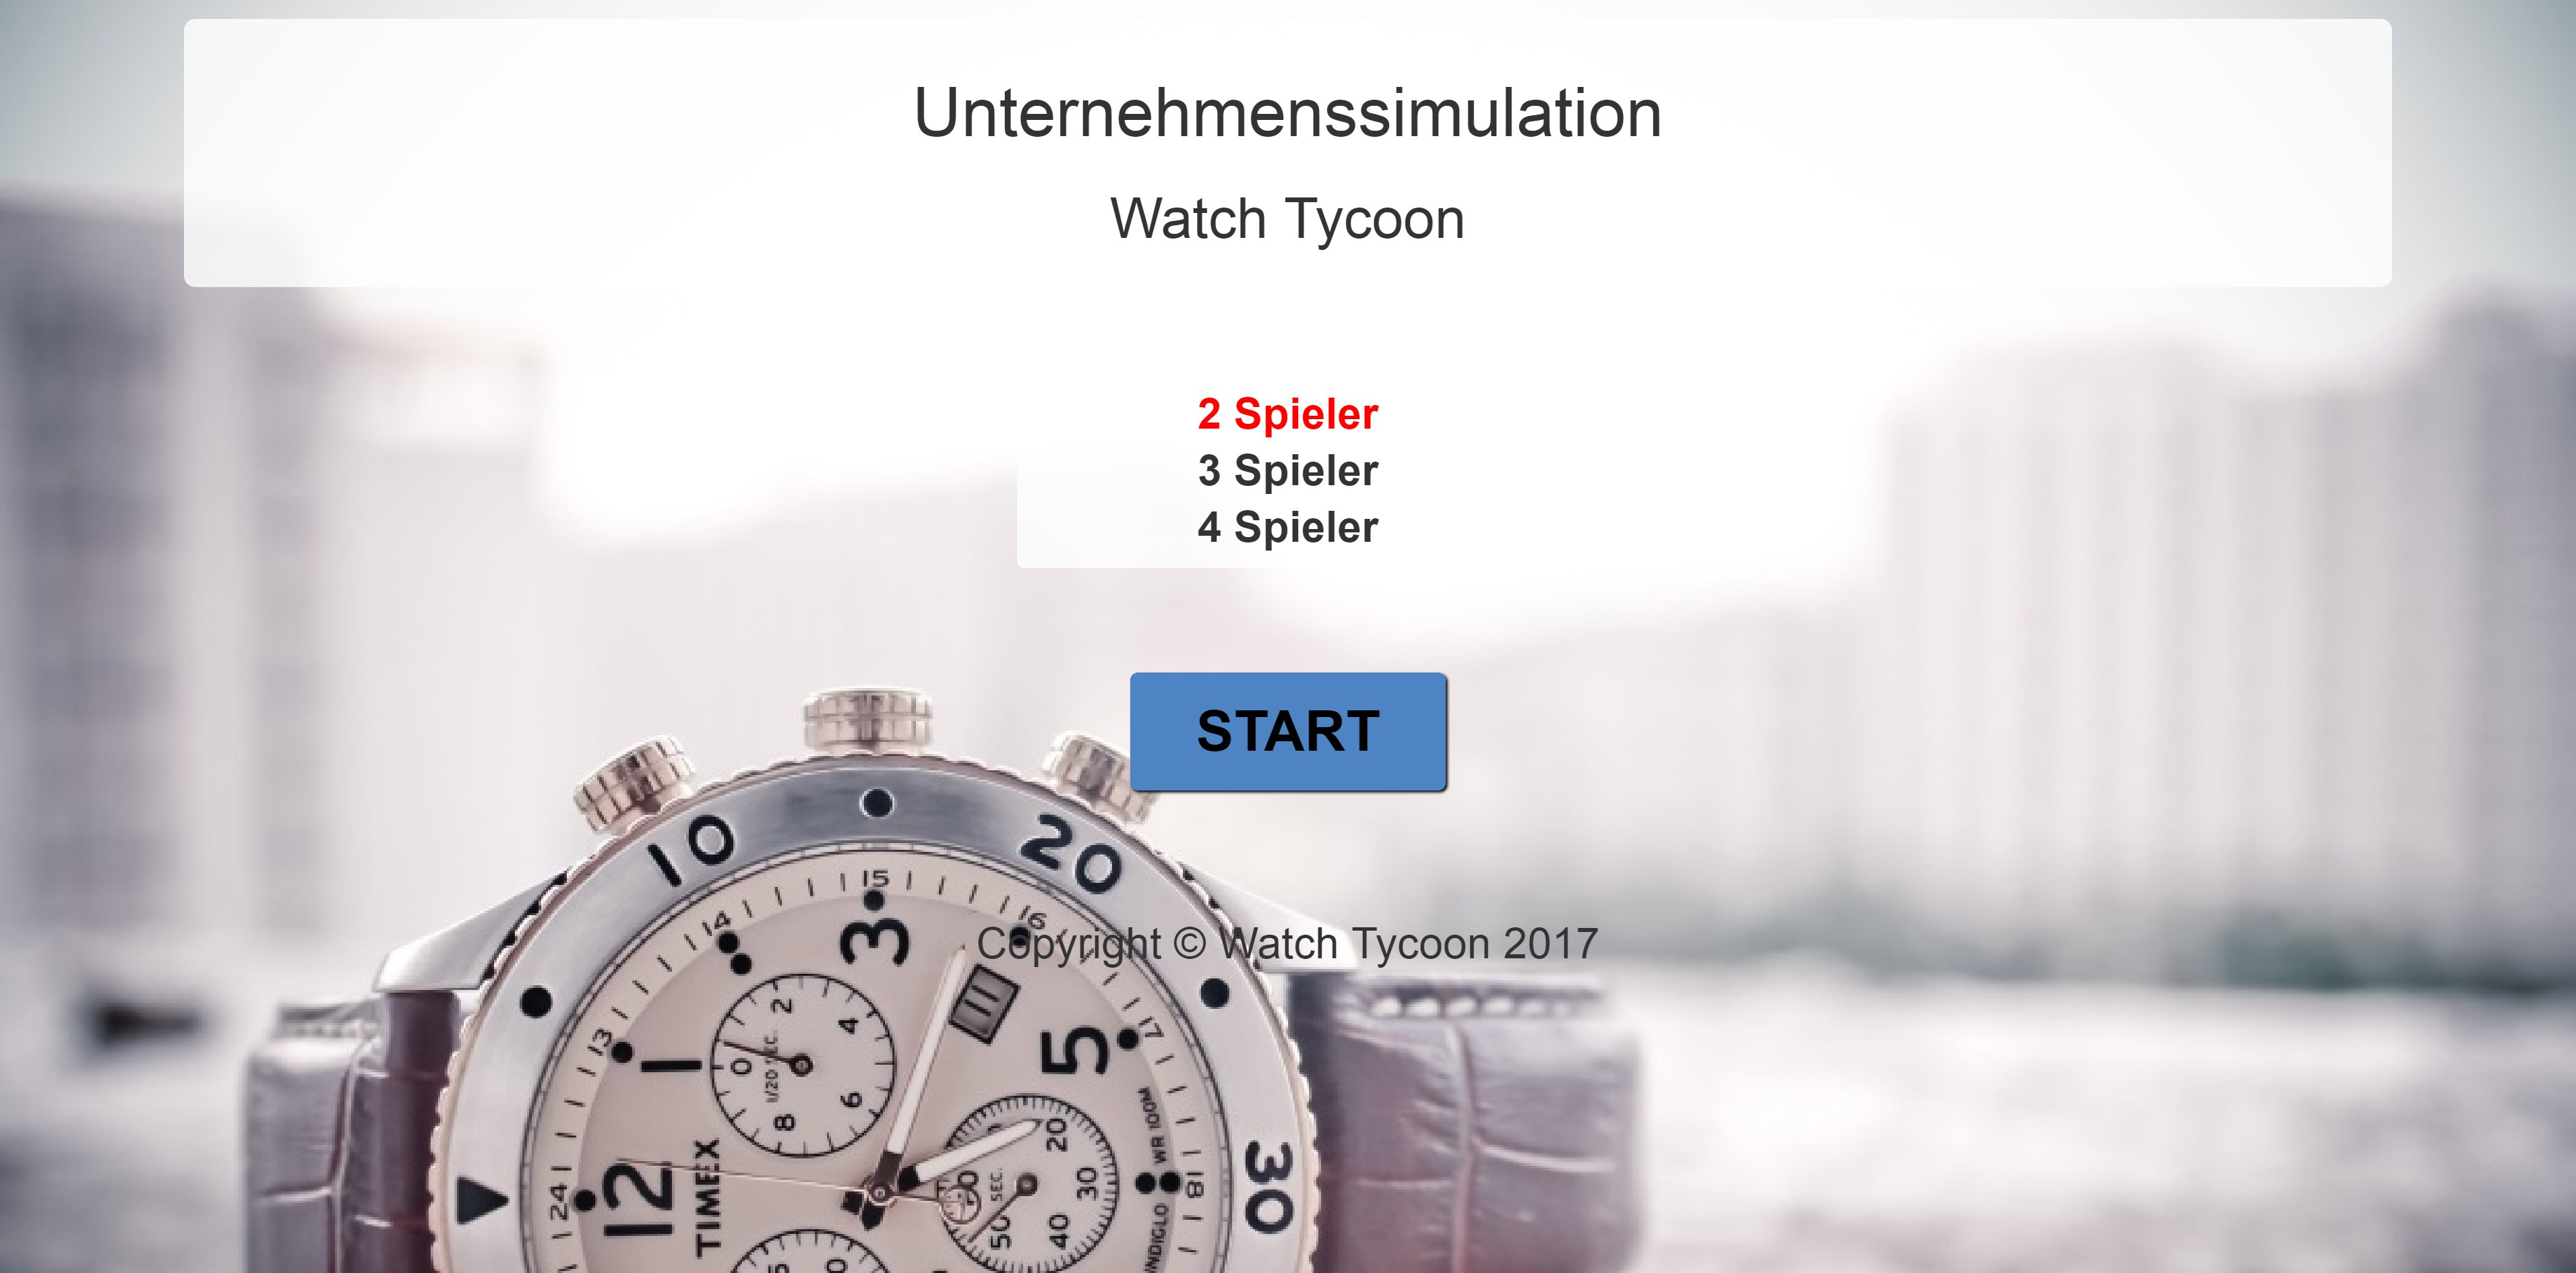
\includegraphics[scale=0.1]{img/bilder_layout/Spiel1.jpg}
	\label{fig:abb16}
	\caption{UI: Einstiegsbildschirm} 
\end{figure}

\begin{figure} [!h]
\begin{minipage}{\textwidth}
Jeder Spieler bekommt in der 1. Runde die Auswahl zwischen den drei Segmenten und kann daraus ein Segment auswählen.\\
\end{minipage}
	\centering
	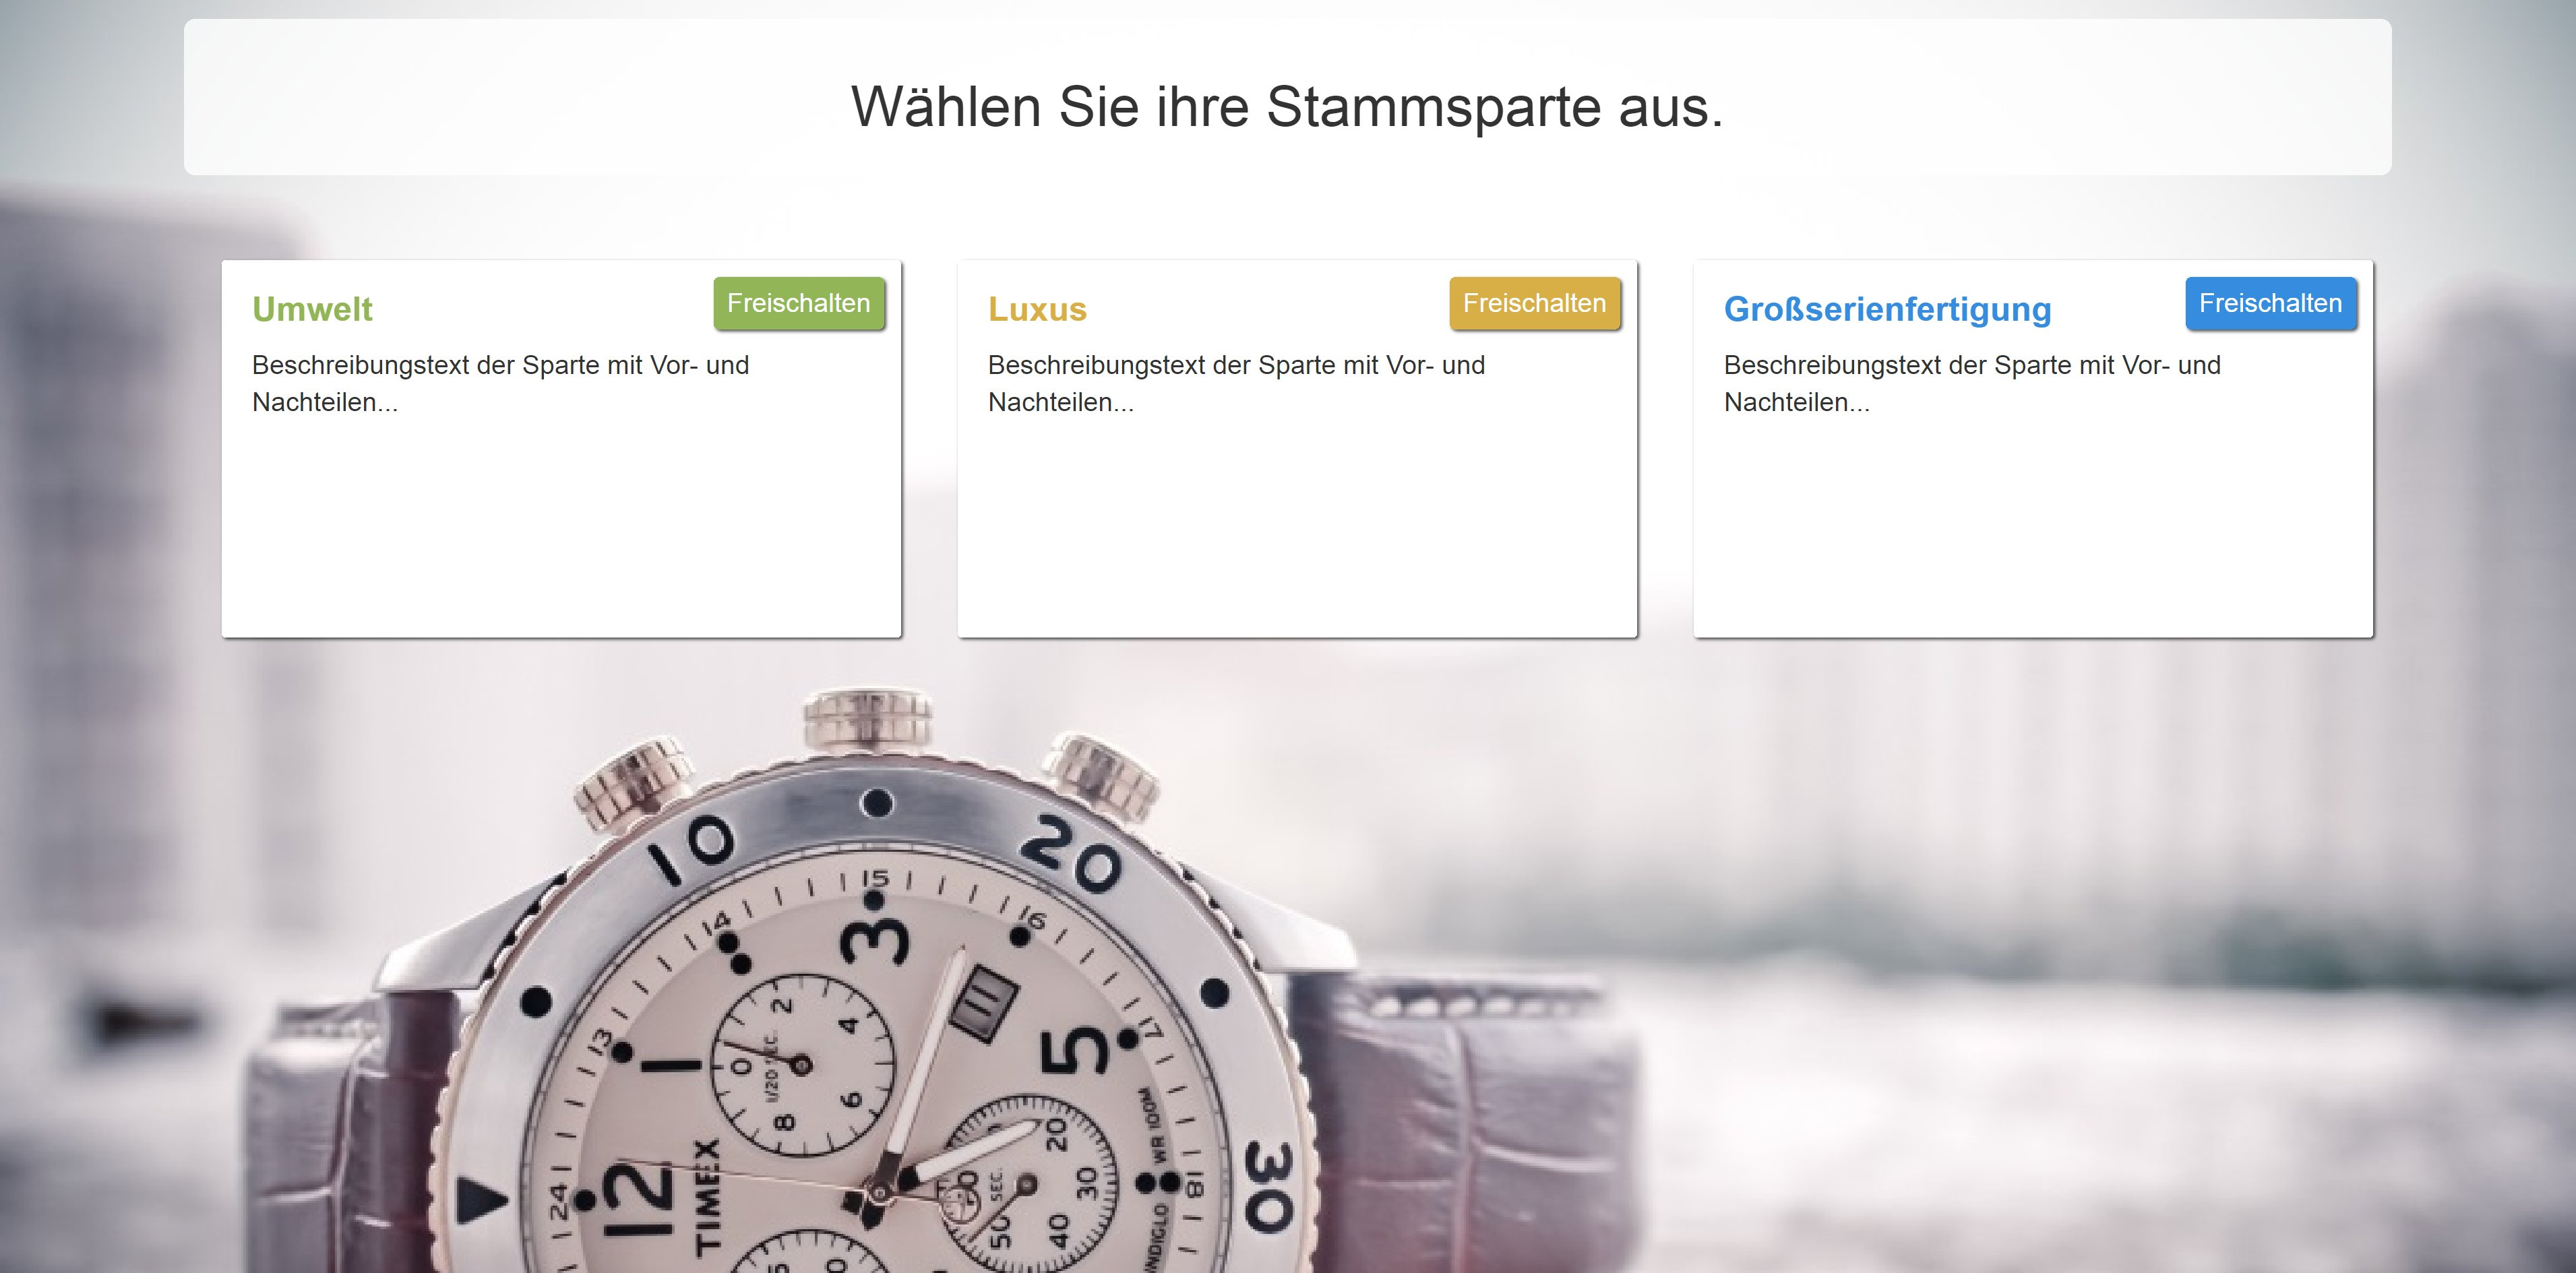
\includegraphics[scale=0.1]{img/bilder_layout/Spiel2.jpg}
	\label{fig:abb17}
	\caption{UI: Segmentauswahl für Spieler X} 
\end{figure}

\begin{figure}
\begin{minipage}{\textwidth}
Hier erhält der Spieler eine Übersicht über seine max. drei Uhren und deren Materialien.\\
\end{minipage}
	\centering
	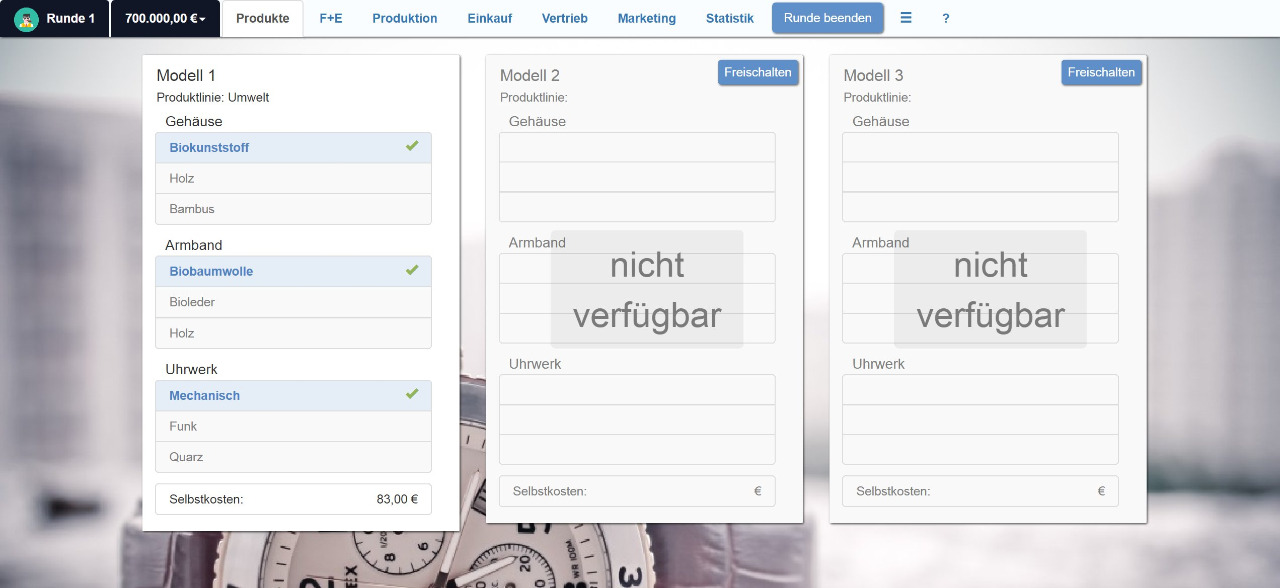
\includegraphics[scale=0.3]{img/bilder_layout/produkte.jpeg}
	\label{fig:abb18}
	\caption{UI: Übersicht der Produkte}  
\end{figure}

\begin{figure}
	\begin{minipage}{\textwidth}
Zusätzlich erhält man mit einem \enquote{Klick} auf das Kapital werden die verschiedenen Bestände angezeigt.\\
	\end{minipage}
	\centering
	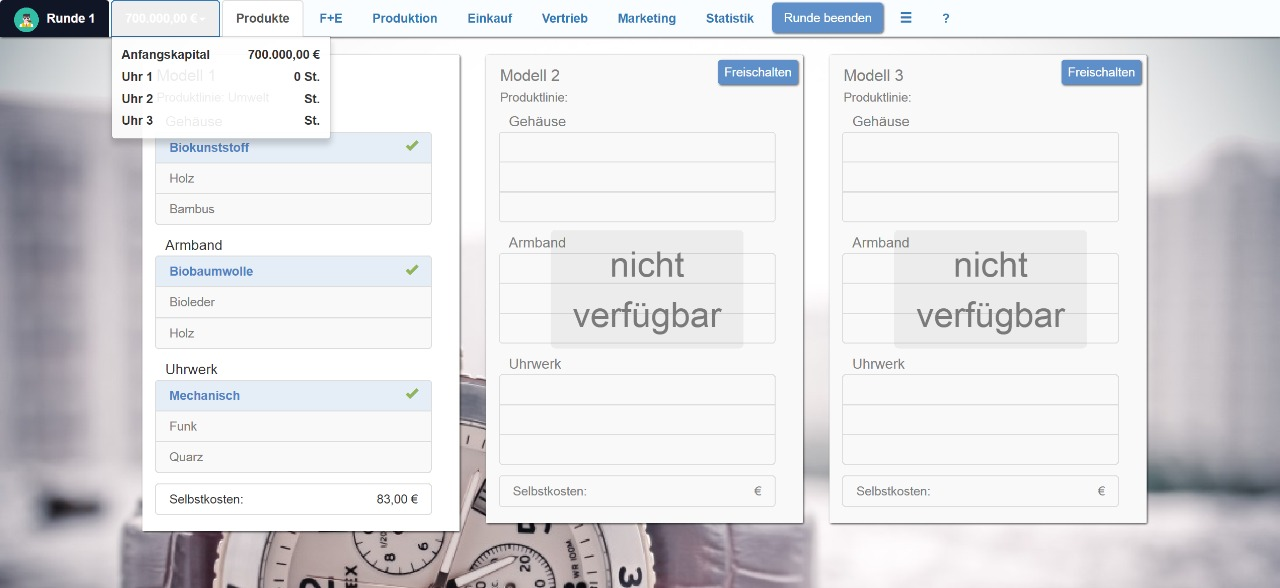
\includegraphics[scale=0.3]{img/bilder_layout/spieler.jpeg}
	\label{fig:abb19}
	\caption{UI: Bestandsübersicht}
\end{figure}

\begin{figure}
\begin{minipage}{\textwidth}
Der Spieler kann Entwicklungen an seiner Uhr durchführen und hochwertigere Materialien erforschen.\\
\end{minipage}
	\centering
	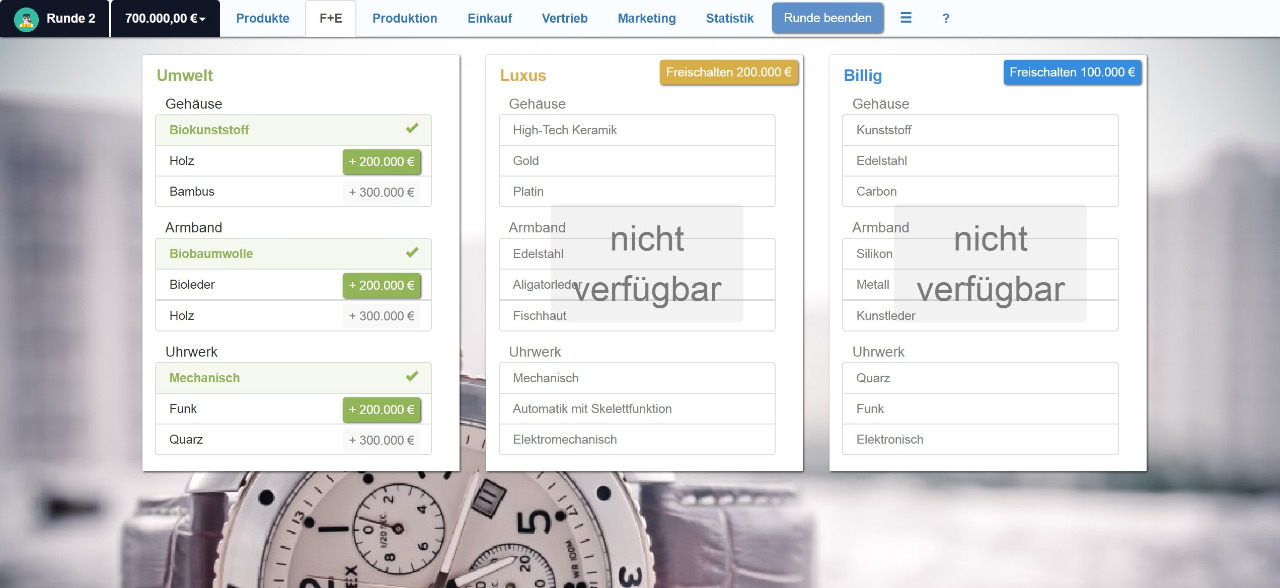
\includegraphics[scale=0.3]{img/bilder_layout/fe.jpeg}
	\label{fig:abb20}
	\caption{UI: Übersicht F\&E} 
\end{figure}

\begin{figure}
\begin{minipage}{\textwidth}
Im Reiter Produktion können weitere Produktionsstraßen und Produktionserweiterungen gekauft werden.\\
\end{minipage}
	\centering
	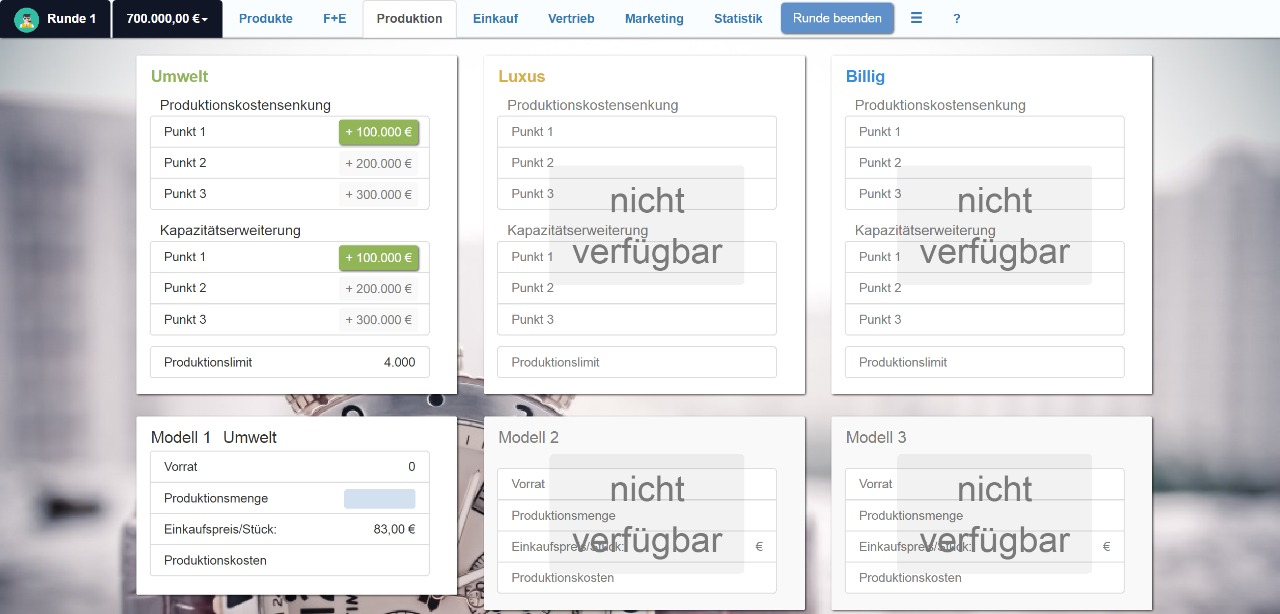
\includegraphics[scale=0.3]{img/bilder_layout/produktion.jpeg}
	\label{fig:abb21}
	\caption{UI: Übersicht Produktion} 
\end{figure}

\begin{figure}
\begin{minipage}{\textwidth}
Der Einkauf zeigt die jeweiligen Teilepreise für die Herstellung der Uhr.\\
\end{minipage}
	\centering
	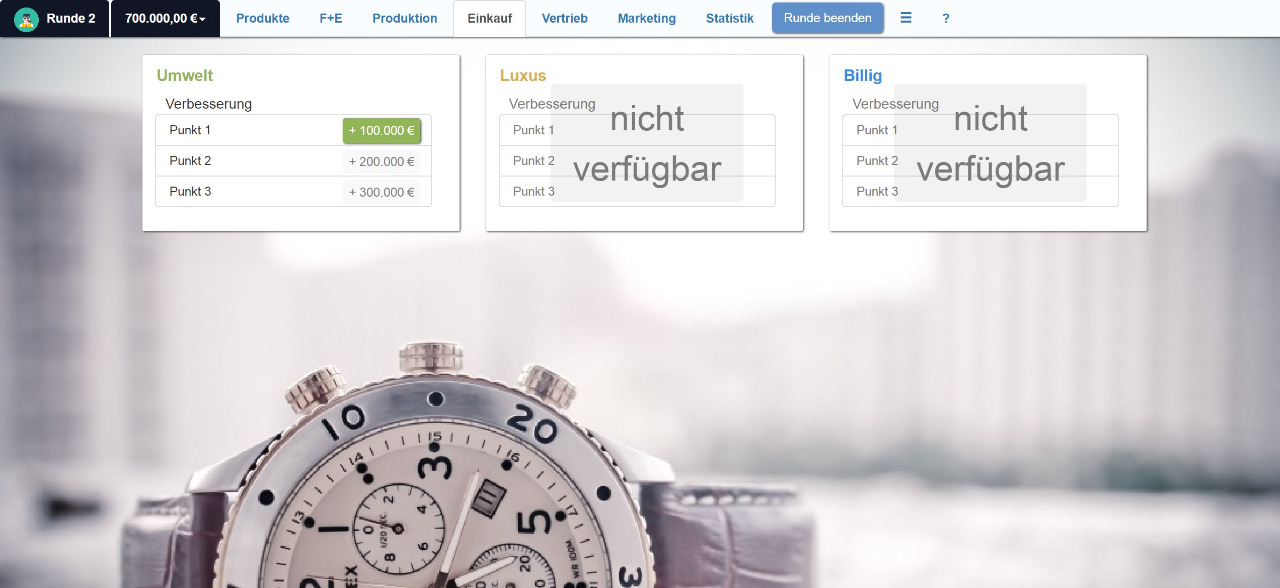
\includegraphics[scale=0.3]{img/bilder_layout/einkauf.jpeg}
	\label{fig:abb22}
	\caption{UI: Übersicht Einkauf} 
\end{figure}

\begin{figure}
\begin{minipage}{\textwidth}
In den Spalten \enquote{Verkaufspreis} und \enquote{geplanter Absatz} können die jeweiligen Werte beliebig je nach Verfügbarkeit eingegeben werden.\\
\end{minipage}
	\centering
	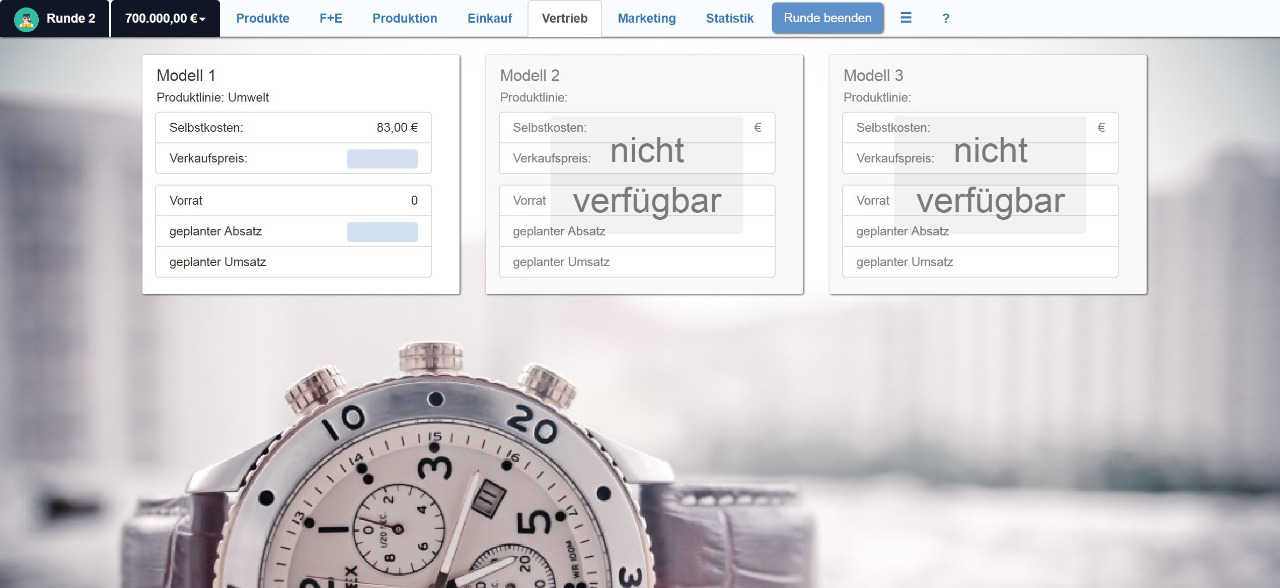
\includegraphics[scale=0.3]{img/bilder_layout/vertrieb.jpeg}
	\label{fig:abb23}
	\caption{UI: Übersicht Vertrieb} 
\end{figure}

\begin{figure}
\begin{minipage}{\textwidth}
Im Marketingbereich können verschiedene Unternehmens- oder Uhren-spezifische Kampagnen gestartet und deren Auswirkung eingesehen werden.\\
\end{minipage}
	\centering
	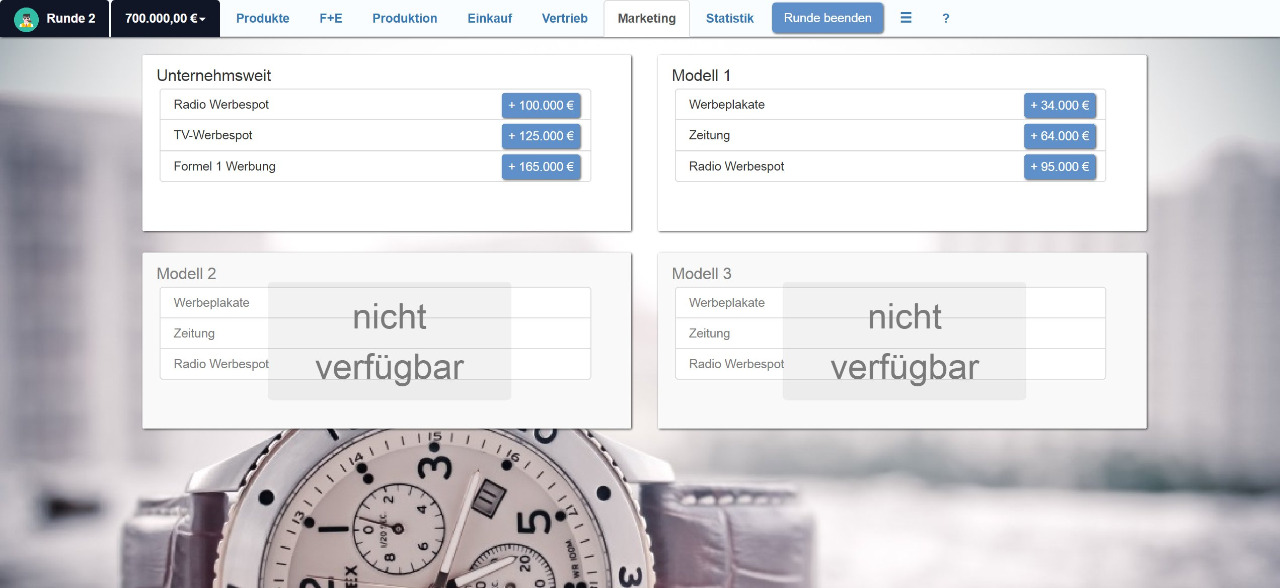
\includegraphics[scale=0.3]{img/bilder_layout/marketing.jpeg}
	\label{fig:abb24}
	\caption{UI: Übersicht Marketing} 
\end{figure}

\begin{figure}
	\begin{minipage}{\textwidth}
Im letzten Reiter Statistik wird eine kleine Übersicht über alle wichtigen Spiel-Informationen geliefert.\\
	\end{minipage}
	\centering
	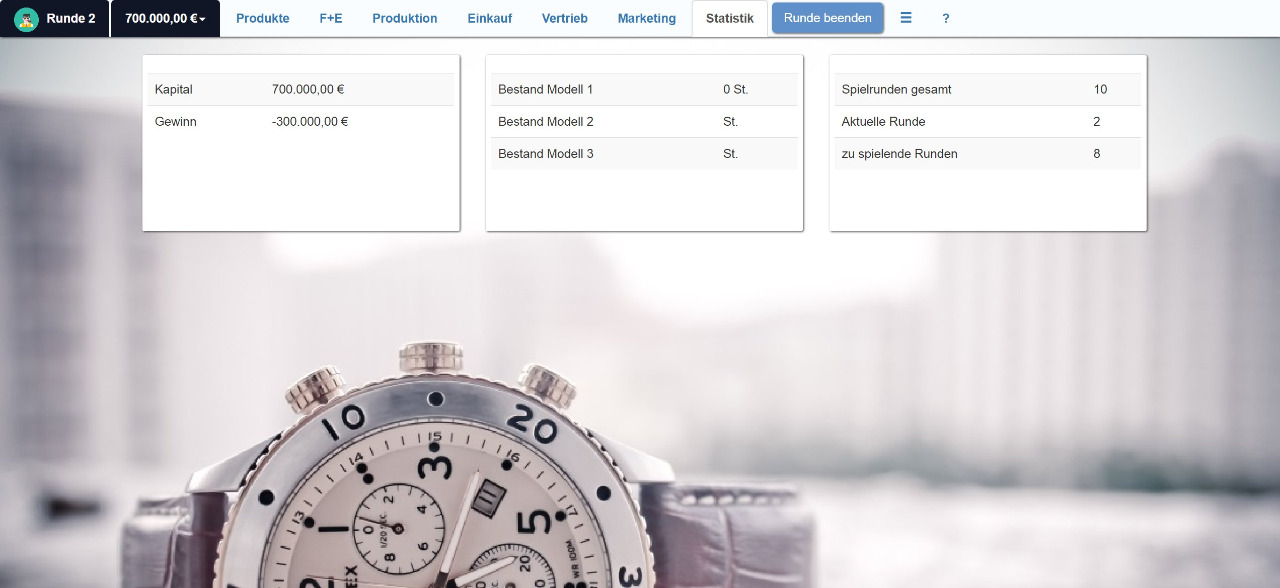
\includegraphics[scale=0.3]{img/bilder_layout/statistik.jpeg}
	\label{fig:abb25}
	\caption{UI: Übersicht Statistik} 
\end{figure}

\begin{figure}
	\begin{minipage}{\textwidth}
Eine kleine Platzierungsübersicht gibt es am Ende auch.\\
	\end{minipage}
	\centering
	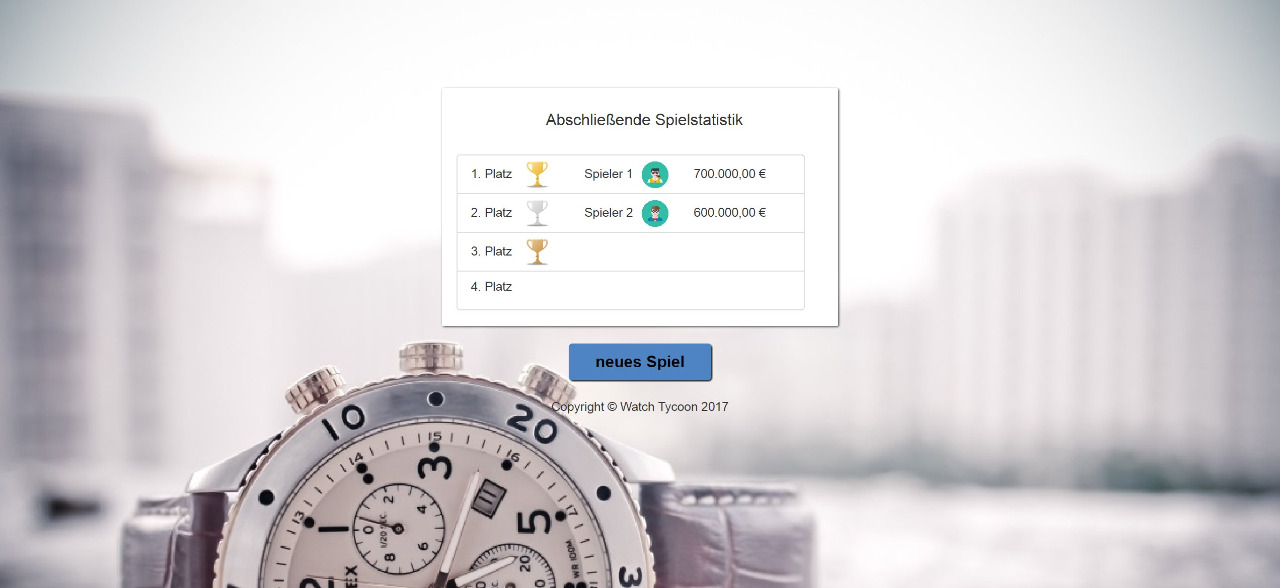
\includegraphics[scale=0.3]{img/bilder_layout/sieger.jpeg}
	\label{fig:abb26}
	\caption{UI: Übersicht Sieger}
\end{figure}